% Options for packages loaded elsewhere
\PassOptionsToPackage{unicode}{hyperref}
\PassOptionsToPackage{hyphens}{url}
\PassOptionsToPackage{dvipsnames,svgnames,x11names}{xcolor}
%
\documentclass[
]{article}
\usepackage{amsmath,amssymb}
\usepackage{iftex}
\ifPDFTeX
  \usepackage[T1]{fontenc}
  \usepackage[utf8]{inputenc}
  \usepackage{textcomp} % provide euro and other symbols
\else % if luatex or xetex
  \usepackage{unicode-math} % this also loads fontspec
  \defaultfontfeatures{Scale=MatchLowercase}
  \defaultfontfeatures[\rmfamily]{Ligatures=TeX,Scale=1}
\fi
\usepackage{lmodern}
\ifPDFTeX\else
  % xetex/luatex font selection
\fi
% Use upquote if available, for straight quotes in verbatim environments
\IfFileExists{upquote.sty}{\usepackage{upquote}}{}
\IfFileExists{microtype.sty}{% use microtype if available
  \usepackage[]{microtype}
  \UseMicrotypeSet[protrusion]{basicmath} % disable protrusion for tt fonts
}{}
\makeatletter
\@ifundefined{KOMAClassName}{% if non-KOMA class
  \IfFileExists{parskip.sty}{%
    \usepackage{parskip}
  }{% else
    \setlength{\parindent}{0pt}
    \setlength{\parskip}{6pt plus 2pt minus 1pt}}
}{% if KOMA class
  \KOMAoptions{parskip=half}}
\makeatother
\usepackage{xcolor}
\usepackage{longtable,booktabs,array}
\usepackage{calc} % for calculating minipage widths
% Correct order of tables after \paragraph or \subparagraph
\usepackage{etoolbox}
\makeatletter
\patchcmd\longtable{\par}{\if@noskipsec\mbox{}\fi\par}{}{}
\makeatother
% Allow footnotes in longtable head/foot
\IfFileExists{footnotehyper.sty}{\usepackage{footnotehyper}}{\usepackage{footnote}}
\makesavenoteenv{longtable}
\usepackage{graphicx}
\makeatletter
\def\maxwidth{\ifdim\Gin@nat@width>\linewidth\linewidth\else\Gin@nat@width\fi}
\def\maxheight{\ifdim\Gin@nat@height>\textheight\textheight\else\Gin@nat@height\fi}
\makeatother
% Scale images if necessary, so that they will not overflow the page
% margins by default, and it is still possible to overwrite the defaults
% using explicit options in \includegraphics[width, height, ...]{}
\setkeys{Gin}{width=\maxwidth,height=\maxheight,keepaspectratio}
% Set default figure placement to htbp
\makeatletter
\def\fps@figure{htbp}
\makeatother
\usepackage{svg}
\setlength{\emergencystretch}{3em} % prevent overfull lines
\providecommand{\tightlist}{%
  \setlength{\itemsep}{0pt}\setlength{\parskip}{0pt}}
\setcounter{secnumdepth}{5}
% definitions for citeproc citations
\NewDocumentCommand\citeproctext{}{}
\NewDocumentCommand\citeproc{mm}{%
  \begingroup\def\citeproctext{#2}\cite{#1}\endgroup}
\makeatletter
 % allow citations to break across lines
 \let\@cite@ofmt\@firstofone
 % avoid brackets around text for \cite:
 \def\@biblabel#1{}
 \def\@cite#1#2{{#1\if@tempswa , #2\fi}}
\makeatother
\newlength{\cslhangindent}
\setlength{\cslhangindent}{1.5em}
\newlength{\csllabelwidth}
\setlength{\csllabelwidth}{3em}
\newenvironment{CSLReferences}[2] % #1 hanging-indent, #2 entry-spacing
 {\begin{list}{}{%
  \setlength{\itemindent}{0pt}
  \setlength{\leftmargin}{0pt}
  \setlength{\parsep}{0pt}
  % turn on hanging indent if param 1 is 1
  \ifodd #1
   \setlength{\leftmargin}{\cslhangindent}
   \setlength{\itemindent}{-1\cslhangindent}
  \fi
  % set entry spacing
  \setlength{\itemsep}{#2\baselineskip}}}
 {\end{list}}
\usepackage{calc}
\newcommand{\CSLBlock}[1]{\hfill\break\parbox[t]{\linewidth}{\strut\ignorespaces#1\strut}}
\newcommand{\CSLLeftMargin}[1]{\parbox[t]{\csllabelwidth}{\strut#1\strut}}
\newcommand{\CSLRightInline}[1]{\parbox[t]{\linewidth - \csllabelwidth}{\strut#1\strut}}
\newcommand{\CSLIndent}[1]{\hspace{\cslhangindent}#1}
%% personal sizes for drafts
\topmargin=-0.5in
\textheight=9.2in
\oddsidemargin=-0.2in
\evensidemargin=0.0in
\textwidth=6.90in
\parindent=30pt
\parskip=3pt
\headheight=15pt
\reversemarginpar
\marginparwidth=.75in

%\setkeys{Gin}{width=.75\textwidth,keepaspectratio}


\makeatletter
\@ifpackageloaded{subfig}{}{\usepackage{subfig}}
\@ifpackageloaded{caption}{}{\usepackage{caption}}
\captionsetup[subfloat]{margin=0.5em}
\AtBeginDocument{%
\renewcommand*\figurename{Figure}
\renewcommand*\tablename{Table}
}
\AtBeginDocument{%
\renewcommand*\listfigurename{List of Figures}
\renewcommand*\listtablename{List of Tables}
}
\newcounter{pandoccrossref@subfigures@footnote@counter}
\newenvironment{pandoccrossrefsubfigures}{%
\setcounter{pandoccrossref@subfigures@footnote@counter}{0}
\begin{figure}\centering%
\gdef\global@pandoccrossref@subfigures@footnotes{}%
\DeclareRobustCommand{\footnote}[1]{\footnotemark%
\stepcounter{pandoccrossref@subfigures@footnote@counter}%
\ifx\global@pandoccrossref@subfigures@footnotes\empty%
\gdef\global@pandoccrossref@subfigures@footnotes{{##1}}%
\else%
\g@addto@macro\global@pandoccrossref@subfigures@footnotes{, {##1}}%
\fi}}%
{\end{figure}%
\addtocounter{footnote}{-\value{pandoccrossref@subfigures@footnote@counter}}
\@for\f:=\global@pandoccrossref@subfigures@footnotes\do{\stepcounter{footnote}\footnotetext{\f}}%
\gdef\global@pandoccrossref@subfigures@footnotes{}}
\@ifpackageloaded{float}{}{\usepackage{float}}
\floatstyle{ruled}
\@ifundefined{c@chapter}{\newfloat{codelisting}{h}{lop}}{\newfloat{codelisting}{h}{lop}[chapter]}
\floatname{codelisting}{Listing}
\newcommand*\listoflistings{\listof{codelisting}{List of Listings}}
\makeatother
\ifLuaTeX
  \usepackage{selnolig}  % disable illegal ligatures
\fi
\usepackage{bookmark}
\IfFileExists{xurl.sty}{\usepackage{xurl}}{} % add URL line breaks if available
\urlstyle{same}
\hypersetup{
  pdftitle={How to Apply BCM Theory: A Practical Guide Using Amblyopia Treatment as an Example},
  pdfkeywords={bcm, amblyopia, synaptic plasticity},
  colorlinks=true,
  linkcolor={Maroon},
  filecolor={Maroon},
  citecolor={Blue},
  urlcolor={Blue},
  pdfcreator={LaTeX via pandoc}}

\title{How to Apply BCM Theory: A Practical Guide Using Amblyopia
Treatment as an Example}
\author{}
\date{}

\begin{document}
\maketitle
\begin{abstract}
This document should serve as an introduction to the BCM
Theory\textsuperscript{1} of cortical plasticity, using the development
and treatment for amblyopia as the scientific problem to be explored. We
will explore both low-dimensional abstract environments as well as
visual environments based on natural-image input to understand the
dynamics of synaptic plasticity.
\end{abstract}

{
\hypersetup{linkcolor=}
\setcounter{tocdepth}{3}
\tableofcontents
}
\section{Introduction}\label{sec:introduction}

In this introduction, I want to be clear about as many of the underlying
assumptions being made and to highlight where the various results come
from in the simulations. By comparing low-dimension and high-dimension
environments, it's my hope that it will make clearer what sorts of
changes to the input environment will lead to particular dynamics of
synaptic plasticity. Building up one's intuition this way should help in
proposing alternate treatments for amblyopia and understanding how the
parameters of those treatments affect their outcomes.

\subsection{The Neuron}\label{sec:the-neuron}

The BCM theory\textsuperscript{1} of synaptic plasticity starts with a
simplified model of a neuron shown in Figure \ref{fig:simple_neuron}. In
the figure, the model of the neuron has 4 inputs denoted as
\(x_1, x_2, x_3,\) and \(x_4\). These inputs are connected to the cell
via 4 synaptic weights, denoted as \(w_1, w_2, w_3,\) and \(w_4\). The
output of the cell, \(y\), is given as a sum of the input values each
multiplied by the synaptic weight connecting it to the neuron passed
through an output function, often a sigmoid, \(\sigma\): \[
y=\sigma\left(\sum_i x_i w_i \right)
\] In this simple model, the value of neural activity \(x_i=0\) or
\(y=0\) refers to \emph{spontaneous activity}, thus one can have
negative values for this activity representing \emph{below spontaneous}
activity. The sigmoid function is chosen to have the effect of limiting
the spontaneous level of activity, i.e.~the neuron has a larger range of
activity above spontaneous than below it.

The synapse values, \(w_i\), may represent the combination of several
synapses -- including inhibitory synapses -- which implies that the
weights can take on both positive and negative values. The number of
inputs (4 in the case of Figure \ref{fig:simple_neuron}) is arbitrary
and will be different from one environment to another. What is called a
``low-dimensional'' environment is one with few inputs, likewise a
``high-dimensional'' environment will have many (possibly hundreds).

\begin{figure}
\centering
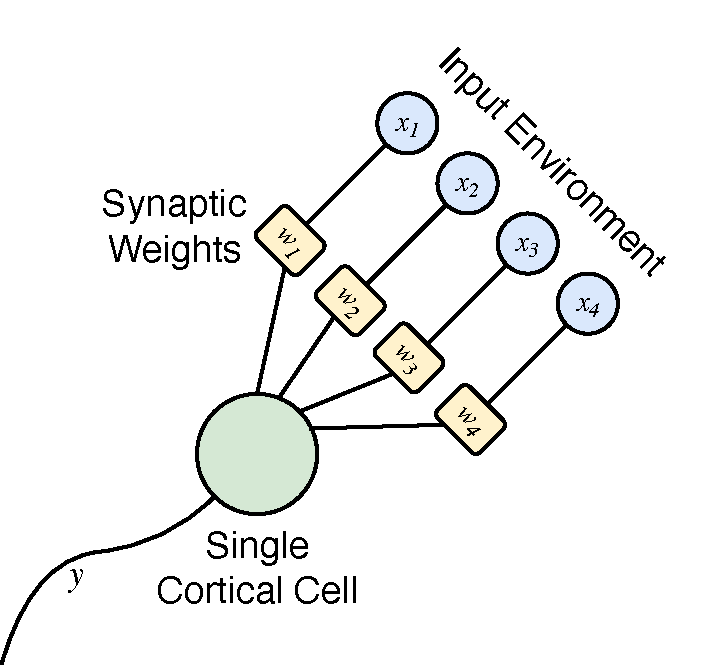
\includegraphics{/Users/bblais/Documents/Git/Amblyopia-Simulation/Manuscript/resources/Simple Neuron.pdf}
\caption{Simple model of a neuron with 4 inputs (\(x_1, x_2, x_3,\) and
\(x_4\)), connecting to the cell via 4 synaptic weights
(\(w_1, w_2, w_3,\) and \(w_4\)), yielding an output
(\(y\)).}\label{fig:simple_neuron}
\end{figure}

\subsection{Plasticity}\label{sec:plasticity}

The BCM theory states that the synaptic weights change depending on the
input to those weights, the output of the neuron, and a sliding
threshold according to the following equations,
\begin{equation}\phantomsection\label{eq:bcm1}{
\frac{dw_i}{dt} = \eta y(y-\theta_M) x_i
}\end{equation}

\begin{equation}\phantomsection\label{eq:bcm2}{
\frac{d\theta_M}{dt} = (y^2-\theta_M)/\tau
}\end{equation}

where is \(x_i\) is the \(i\)th presynaptic input, \(w_i\) is the
\(i\)th synaptic weight, and \(y\) is the postsynaptic output activity.
In Equation \ref{eq:bcm1}, the weights increase if the output, \(y\), is
above the threshold, \(\theta_M\), and decrease if the output is below
the threshold. The sliding threshold, \(\theta_M\), follows postsynaptic
activity in a non-linear way (Equation \ref{eq:bcm2}) and serves to
stabilize any runaway weights and the combination of the two equations
enforces the selectivity property of the BCM neuron\textsuperscript{2}.
The constant, \(\eta\), refers to the learning rate and the constant,
\(\tau\), is what we call the memory constant and is related to the
speed of the sliding threshold. These parameters influence the overall
rate of synaptic plasticity and are generally held constant for any
series of simulations so that relative dynamics can be compared.

The form of the BCM equations is what is called the \emph{quadratic
form} and represents the simplest way of writing the minimum
requirements of the BCM theory, but other forms have also been
explored\textsuperscript{3,4}.

\begin{figure}
\centering
\includesvg{/Users/bblais/Documents/Git/Amblyopia-Simulation/Manuscript/resources/fig-bcm-phi.svg}
\caption{The BCM synaptic modification function. Units are
arbitrary.}\label{fig:fig-bcm-phi.svg}
\end{figure}

\subsection{Selectivity}\label{sec:selectivity}

One of the properties of the BCM learning rule is that in most
environments the neuron becomes \emph{selective} -- it responds to a
small subset of the environment and has low or zero responses to the
rest of the environment. We can see this by looking at the response of
the neuron, \(y\), across the entire environment. Imagine that there are
two possible patterns:

\begin{enumerate}
\def\labelenumi{\arabic{enumi}.}
\tightlist
\item
  input \#1 is \emph{strongly} active and input \#2 is weakly active
\item
  input \#2 is \emph{strongly} active and input \#1 is weakly active
\end{enumerate}

At the start, the BCM neuron responds strongly to both patterns about
the same amount of time. After learning, the BCM becomes selective -- it
responds to only one of the patterns strongly most of the time, and the
other pattern yields a weak response as shown in Figure
\ref{fig:output_dist_2d}. This distribution is \emph{bimodal} -- there
is a cluster of responses above zero and one below zero, separated by a
gap of no responses. When we think of selective responses we often think
in terms of bimodal output distributions. We will see later that this is
not a general property of selective responses, however it is an
intuitive way of thinking about them.

\begin{figure}
\centering
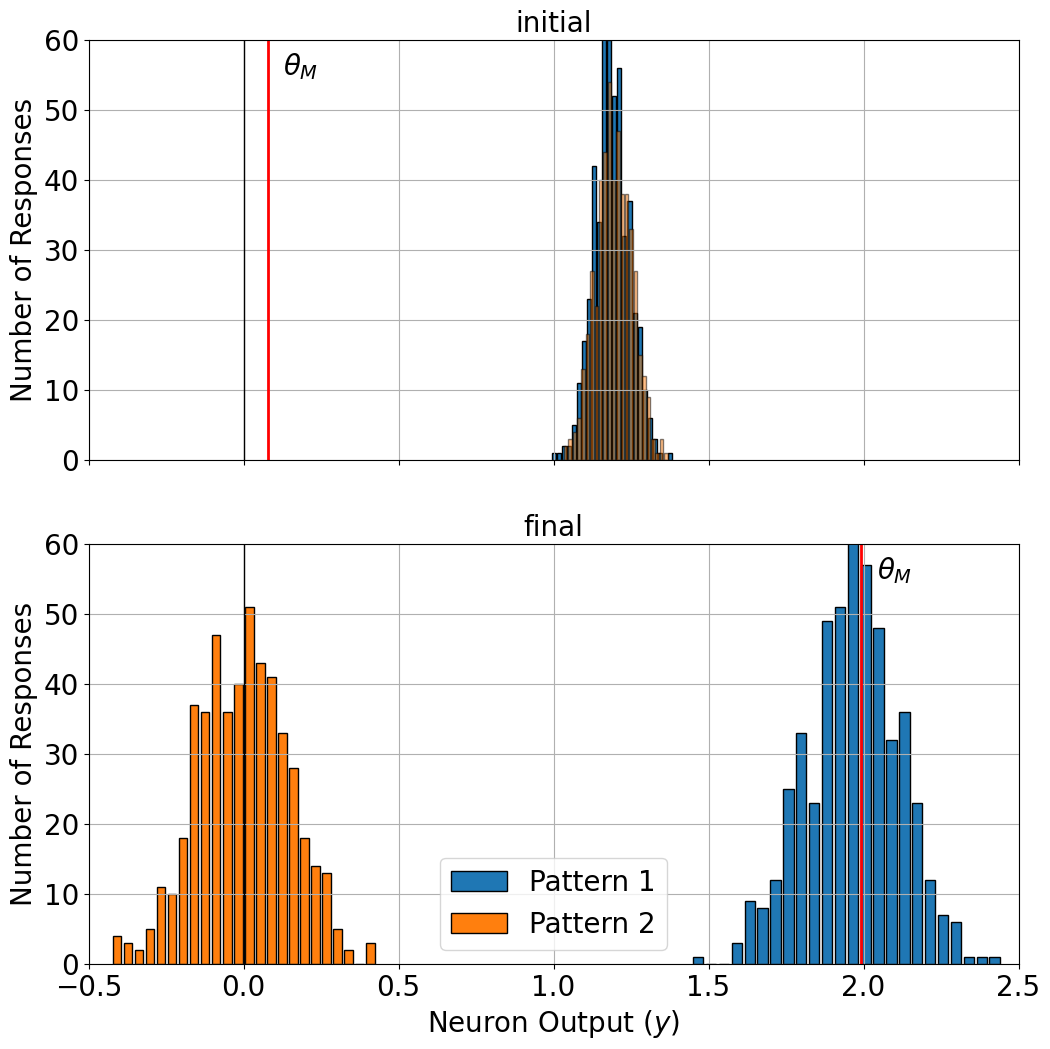
\includegraphics{/Users/bblais/Documents/Git/Amblyopia-Simulation/Manuscript/resources/Pasted image 20240123131156.png}
\caption{The output distribution for a BCM neuron. The initial
distribution (above) shows that the BCM neuron responds strongly to both
patterns about the same amount of time. The final distribution (below)
shows that the BCM neuron responds to only one of the patterns strongly
most of the time, and the other pattern yields a weak response. This
distribution is \emph{bimodal} -- there is a cluster of responses above
zero and one below zero, separated by a gap of no responses. Also notice
that the modification threshold, \(\theta_M\), settles on the value of
the neural output for the selected pattern.}\label{fig:output_dist_2d}
\end{figure}

Geometrically we can plot the input patterns by plotting the activity of
input \#1 on the x-axis and the activity of input \#2 on the y-axis --
this shows 2 primary clusters, as shown in Figure \ref{fig:2d_inputs}.

We can also show the values of the weights as a ``dot'' on this plot,
with the weight for input \#1 on the x-axis and the weight for input \#2
on the y-axis. Visually, it is easier to see it by drawing a line from
the origin to this dot. The output distribution is formed by projecting
a perpendicular from the inputs to this line, as shown in Figure
\ref{fig:2d_initial_weights_outputs} for the initial weights and Figure
\ref{fig:2d_final_weights_outputs} for the final weights. Geometrically,
for the weights to have weak responses to an input pattern then the
weights must be \emph{perpendicular to that input pattern}. One can see
this for the final weights and pattern \#2 in these figures.

\begin{figure}
\centering
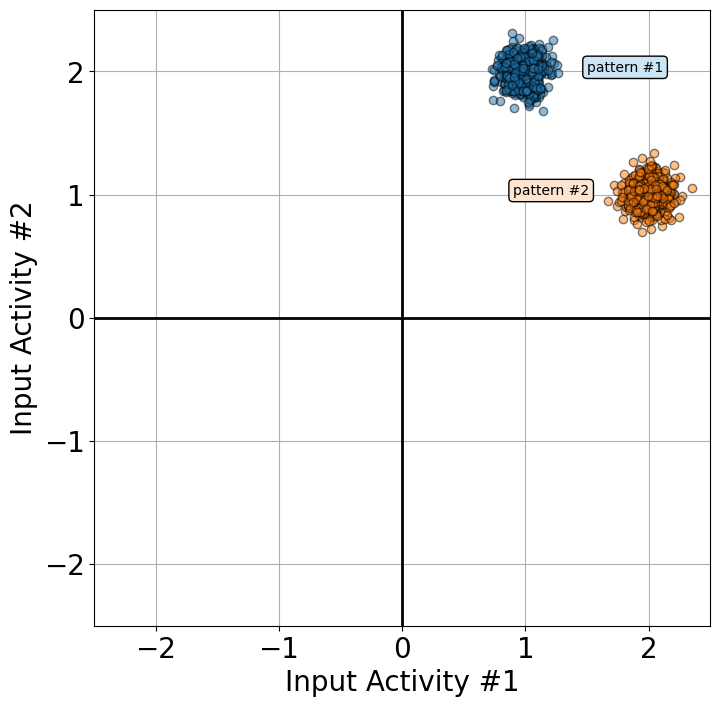
\includegraphics{/Users/bblais/Documents/Git/Amblyopia-Simulation/Manuscript/resources/Pasted image 20240123130523.png}
\caption{2D input environment. .}\label{fig:2d_inputs}
\end{figure}

\begin{figure}
\centering
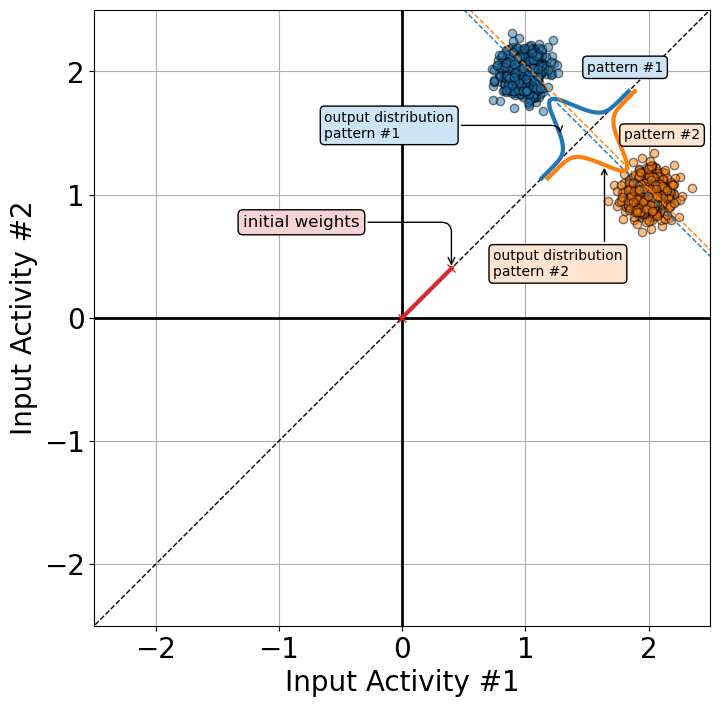
\includegraphics{/Users/bblais/Documents/Git/Amblyopia-Simulation/Manuscript/resources/Pasted image 20240123130539.png}
\caption{Geometric interpretation of the weights and output
distributions for the \emph{initial weights} in a 2D input environment.
.}\label{fig:2d_initial_weights_outputs}
\end{figure}

\begin{figure}
\centering
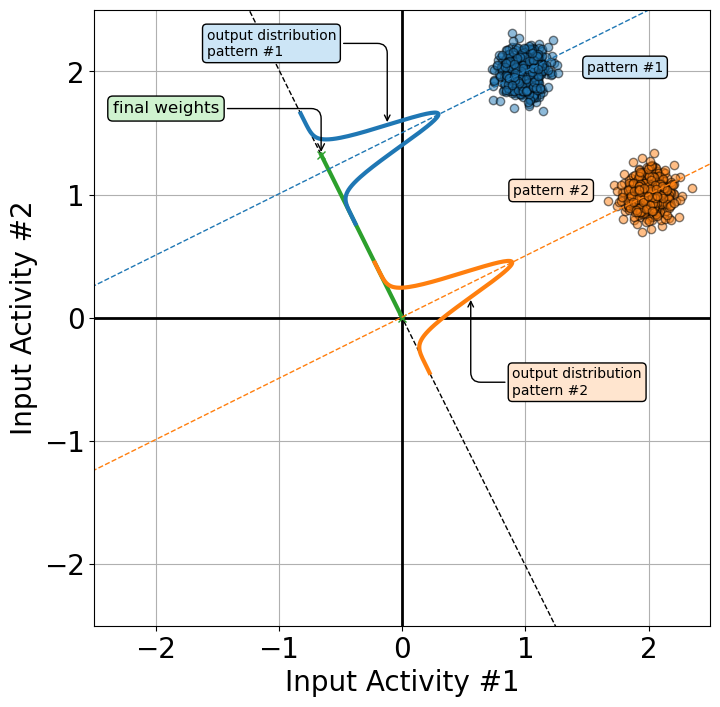
\includegraphics{/Users/bblais/Documents/Git/Amblyopia-Simulation/Manuscript/resources/Pasted image 20240123130559.png}
\caption{Geometric interpretation of the weights and output
distributions for the \emph{final weights} in a 2D input
environment.}\label{fig:2d_final_weights_outputs}
\end{figure}

\subsection{Natural Images}\label{sec:natural-images}

\begin{figure}
\centering
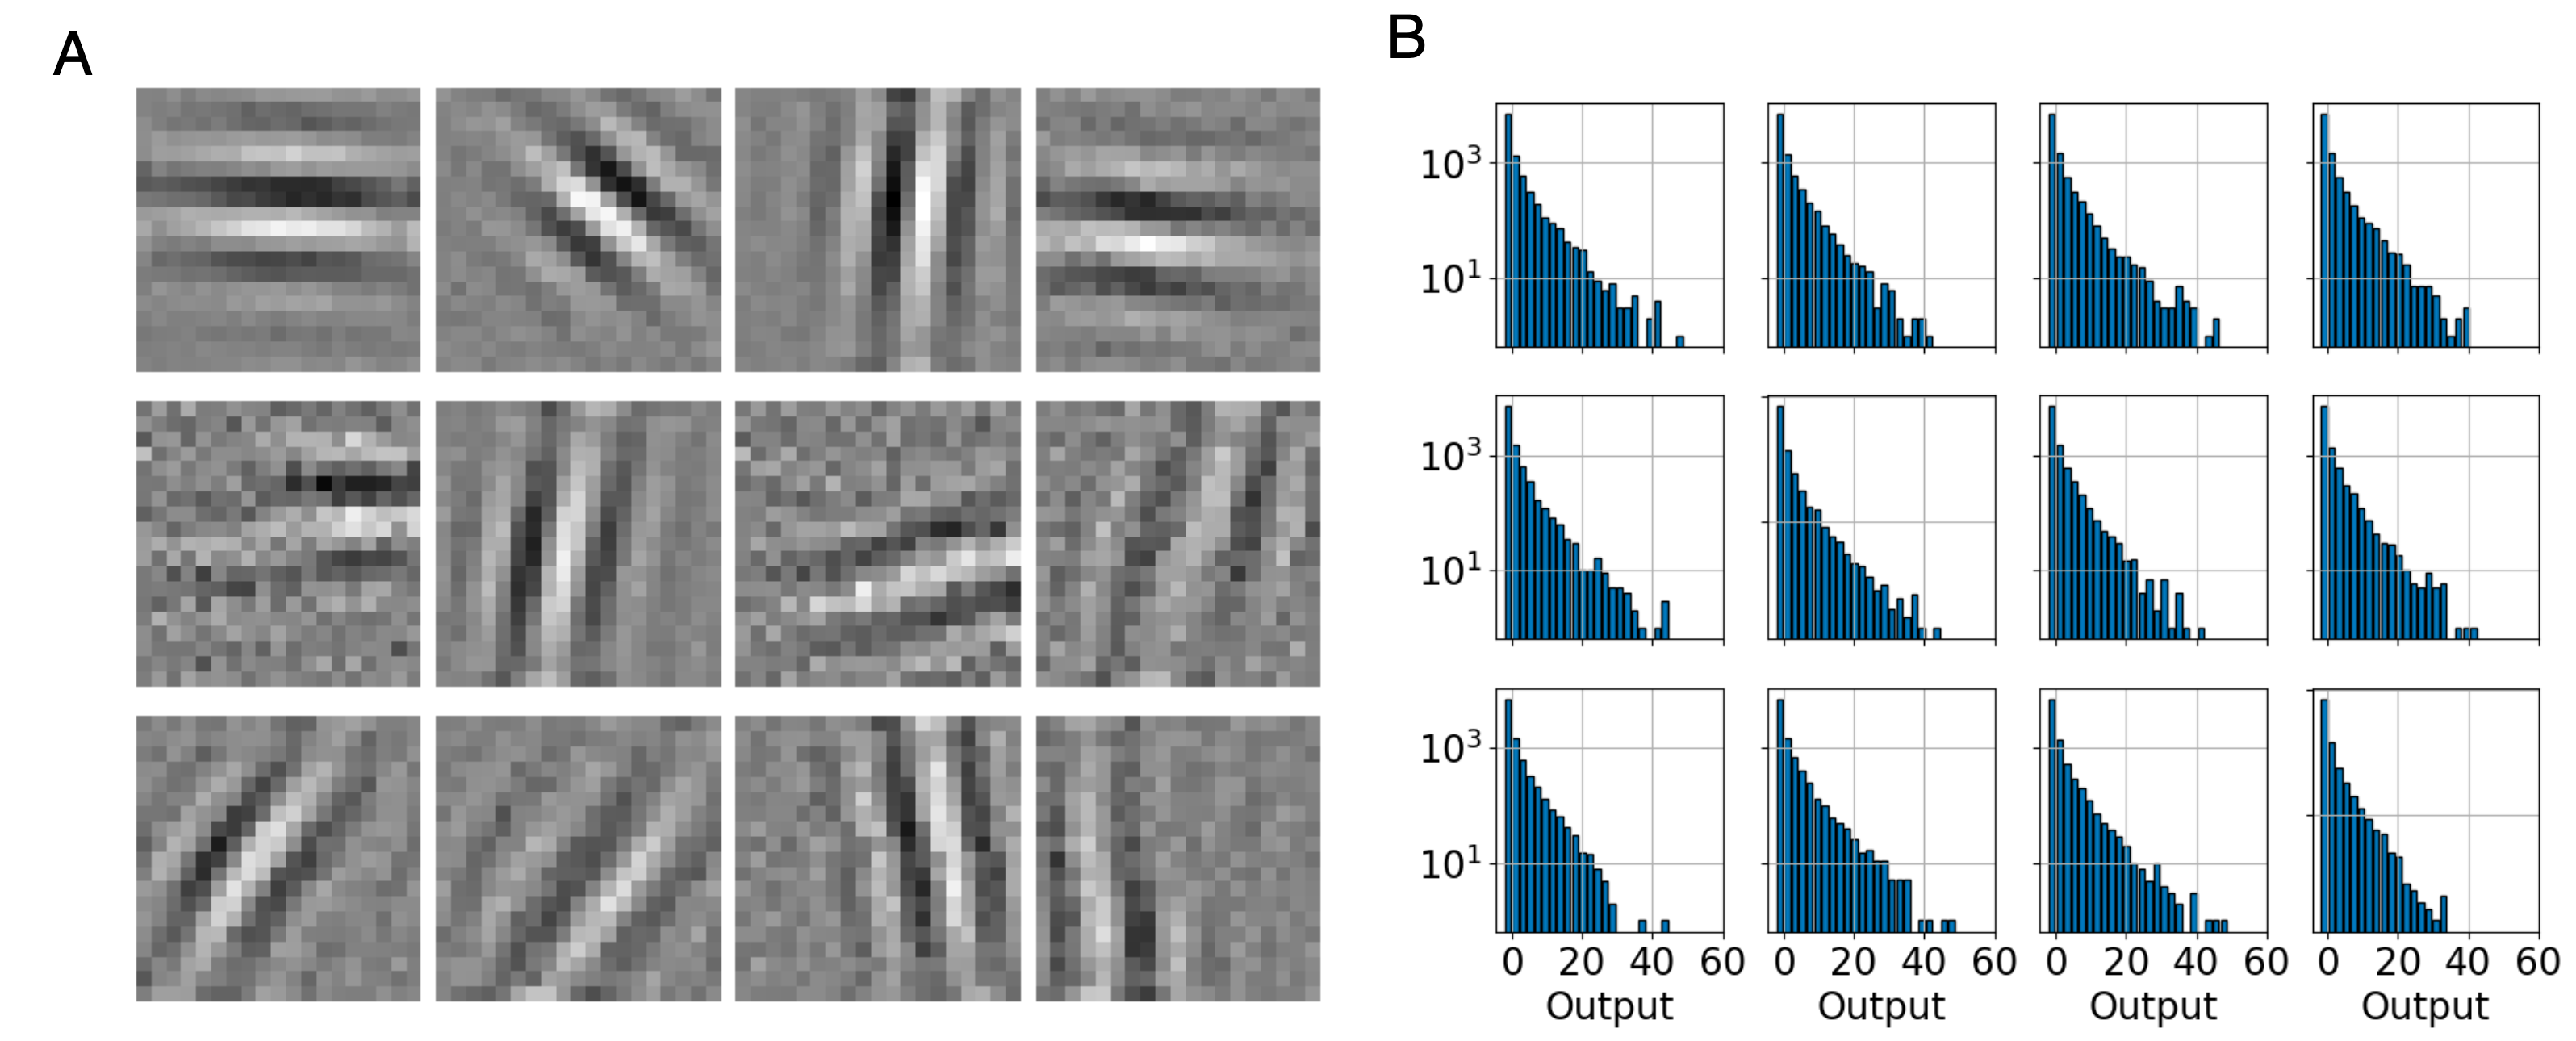
\includegraphics{/Users/bblais/Documents/Git/Amblyopia-Simulation/Manuscript/resources/weights and output distribution natural images.drawio.png}
\caption{Weights (A) and Output distributions (B) for 12 neurons trained
with natural image input patterns. The weights are shown in grayscale,
with black representing low weights and white representing high weights.
The output distribution is shown on a log scale to highlight the few
patterns that yield the strongest
responses.}\label{fig:nat_image_weights_and_output_dist}
\end{figure}

Shown in Figure \ref{fig:nat_image_weights_and_output_dist} are the
weights and output distributions for 12 neurons trained with natural
image input patterns. We easily see that the neurons are selective to
orientation -- the final weights are organized in a line at a particular
orientation. Thus, any input pattern that has that same orientation will
elicit stronger responses because the pattern will align with the strong
weights. Unlike the low dimensional case earlier, the output
distributions for each neuron is \emph{not bimodal}. The output
distribution does not show a cluster above zero and a cluster at zero
with a gap in between, it is smeared out over the entire range of the
responses. What makes the neuron selective is the fact that the vast
bulk of the responses are near zero, and while there is no gap between
low and high responses, the number of patterns yielding strong responses
is very small. Note that the output distributions are being shown on a
log scale, otherwise those strong responses would not even be visible.

This observation means that what BCM neurons select in an environment is
not always \emph{clusters} but a small number of patterns in a sea of
similar patterns. Statistically, this means that BCM is sensitive to
statistics in the input environment beyond separability and 2-point
correlations\textsuperscript{5}. In order to understand the dynamics of
BCM neurons we can explore environments with patterns that don't fall
into neat clusters but instead are spread out with higher order
statistics.

\subsection{Structure vs Noise}\label{sec:structure-vs-noise}

The basic intuition behind the dynamics of the neuron, as it experiences
the changing input environment, comes from an understanding of the
competition between \emph{structure} and \emph{noise}. These terms refer
to the statistics of the input environment and the mathematical form of
the plasticity equations -- different sets of equations will respond to
different forms of \emph{structure} and have different dynamics under
\emph{noise}. This can be used to compare different theories of synaptic
plasticity\textsuperscript{6} but is beyond what we want to discuss
here.

In the case of the BCM theory, the \emph{structure} comes in the form of
an environment with a minority of patterns yielding high responses and
the majority yielding low responses -- the BCM neuron can become
selective in this environment. \emph{Noise} by definition does not have
this property. It is either random variation on top of the structure or
random input without the patterns that can lead to high responses.
Gaussian (i.e.~normal) noise is an example of such variation. Examples
of structure and noise can be visually seen in Figure
\ref{fig:structure_vs_noise}.

\begin{figure}
\centering
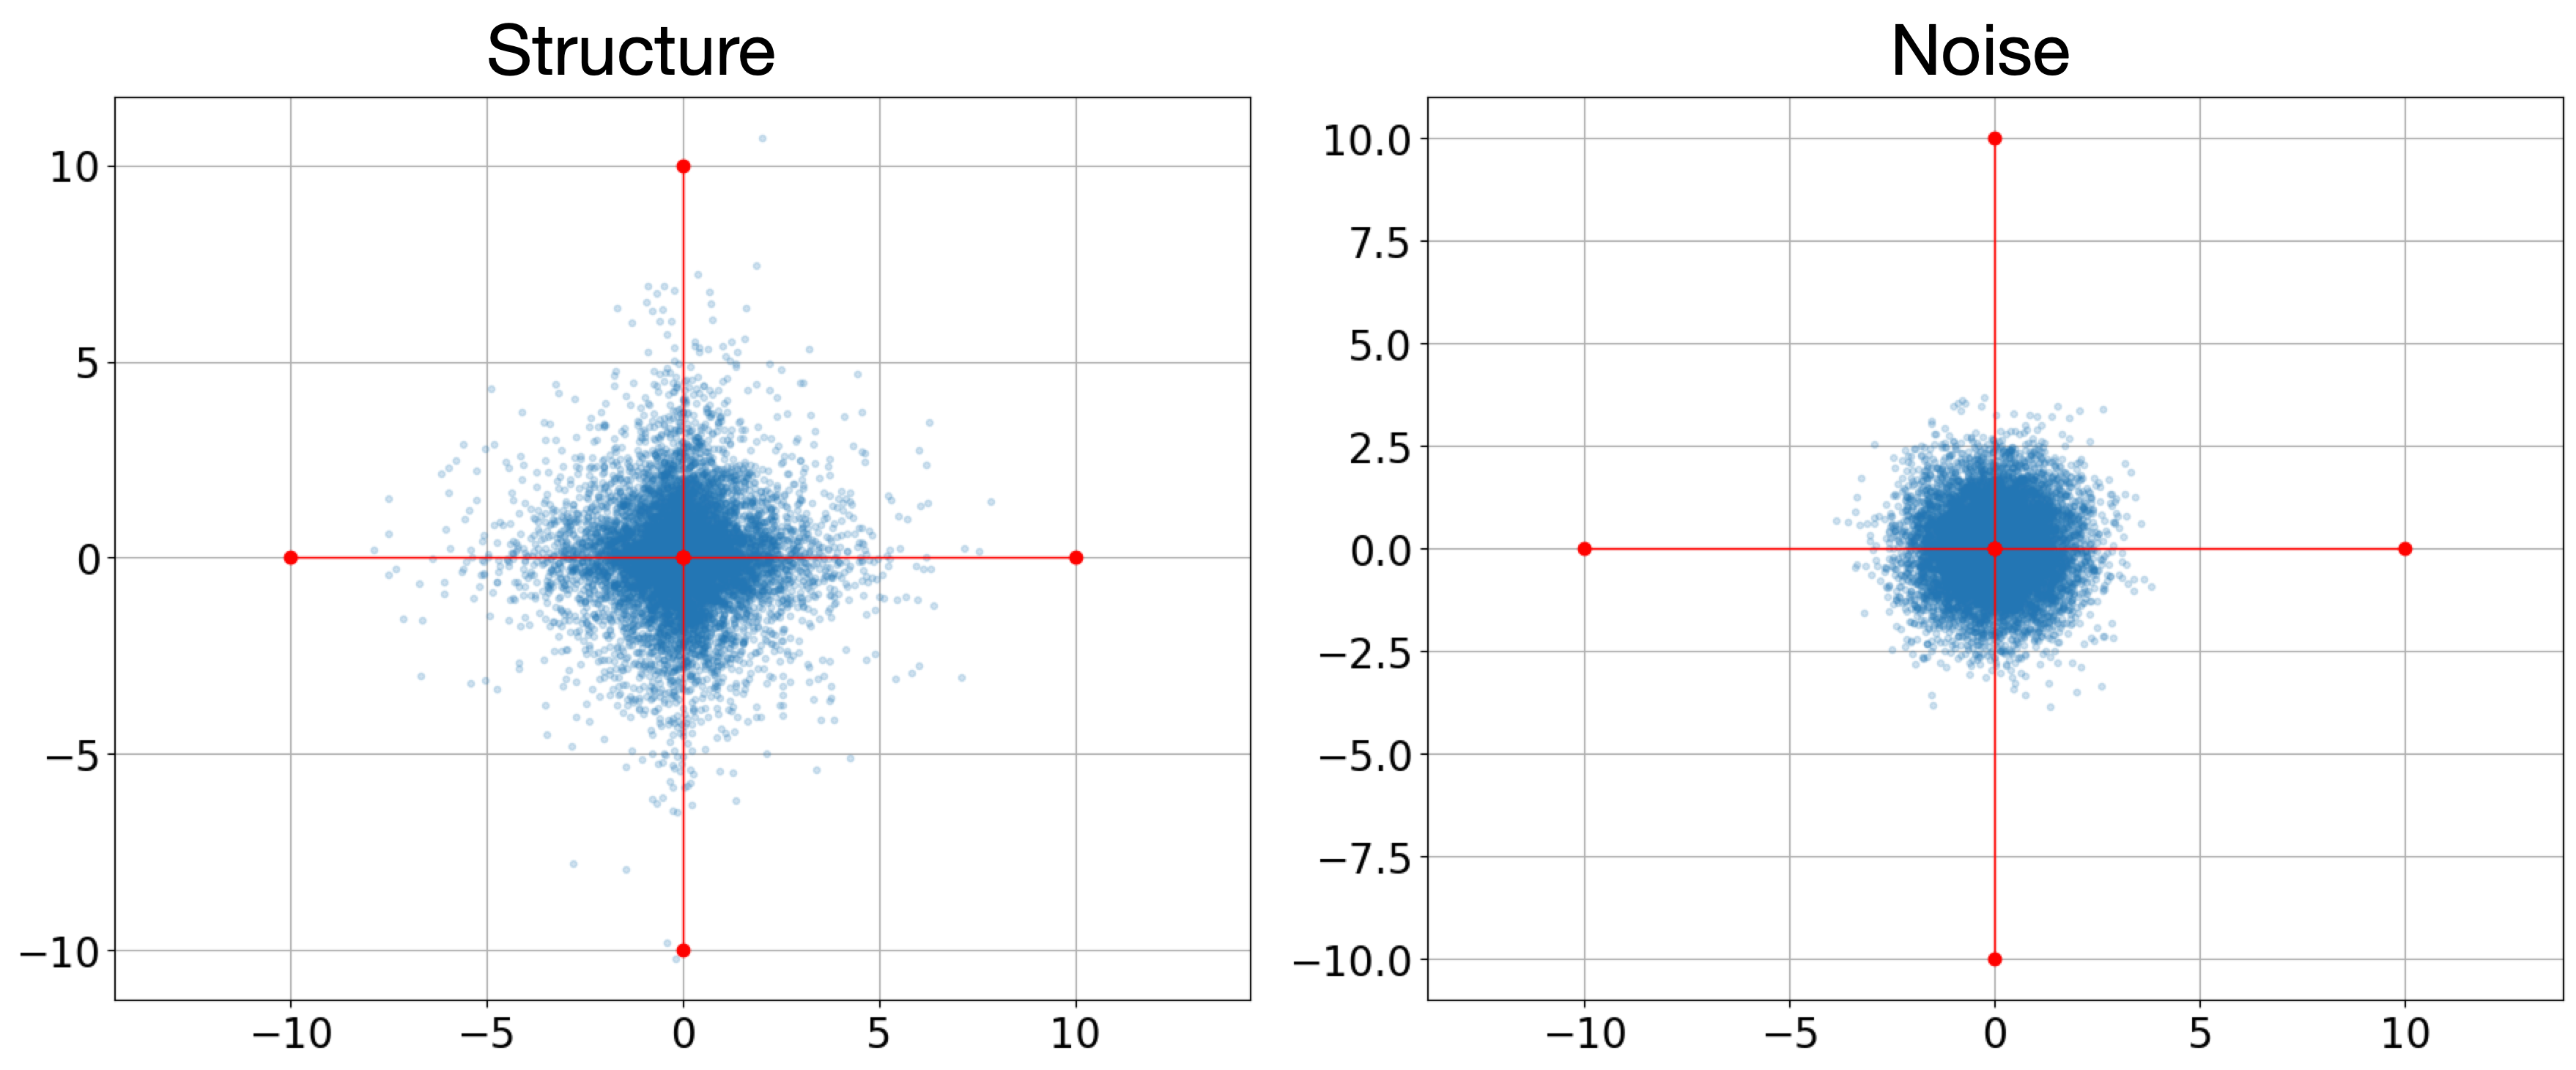
\includegraphics{/Users/bblais/Documents/Git/Amblyopia-Simulation/Manuscript/resources/Pasted image 20240117155651.png}
\caption{Structure (left) and noise (right) for a BCM neuron. Shown on
the axes are the input values for a two-input neuron, the value of input
\(x_1\) shown on the x-axis and input \(x_2\) on the y-axis. Each tiny
blue dot is a snapshot of the activity of \((x_1,x_2)\) at some time.
Over time, as the neuron experiences the environment, the activity plot
fills in the cloud shown. In the case of structure can see a minority
input values that are high, extending out in the x- and y-directions
compared to the noise (right figure) where all directions are equal. In
the structured environment, the weights for the BCM neuron converge to
those directions such that the postsynaptic response is
selective.}\label{fig:structure_vs_noise}
\end{figure}

The \emph{structure} in this case is generated using a distribution
known as the Laplace distribution, or double exponential \[
P(x) \sim e^{-|x|}
\]

The \emph{noise} is generated using a Gaussian or Normal distribution,
\[
P(x) \sim e^{-x^2}
\] Mathematically the difference leads to the Laplace environment having
more values near zero and a significant number of patterns at very high
values (compared to the Gaussian) -- rare patterns. This property of the
Laplace distribution (and some other distributions) is sometimes
referred to as having ``heavy tails''. This mathematical property is
exactly the property the BCM neuron selects for when it learns, so we
expect the BCM to become selective in an environment produced by a
Laplace distribution vs a Gaussian one. We can see the property of rare
input patterns by looking at the distribution itself as in Figure @
\ref{fig:laplace_dist}, shown on a semi-log plot do highlight those
high-value patterns. Compared to a Gaussian, the Laplace distribution
has many more patterns with significantly higher values. The natural
image environment also has a similar structure to the Laplace
environment, even for individual pixels as also shown in Figure @
\ref{fig:laplace_dist}.

\begin{figure}
\centering
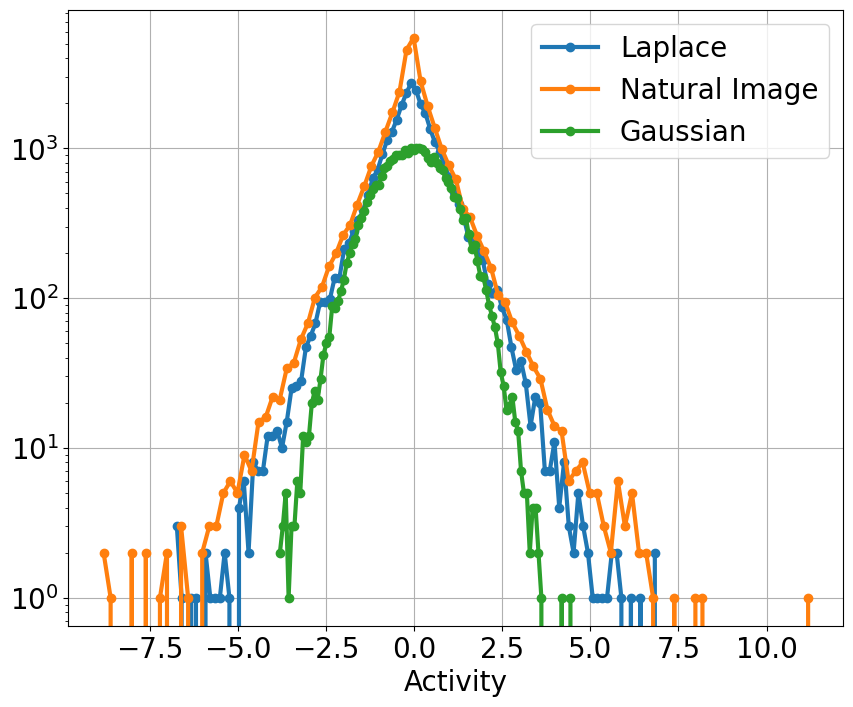
\includegraphics{/Users/bblais/Documents/Git/Amblyopia-Simulation/Manuscript/resources/Pasted image 20240228124006.png}
\caption{Single input (pixel) statistics for the Laplace environment and
the natural image environment compared to Gaussian (i.e.~Normal)
noise.}\label{fig:laplace_dist}
\end{figure}

As the BCM neuron learns, it starts with an output distribution more
similar to a Gaussian and learns to respond more to the rare patterns
with high activity, shown in Figure \ref{fig:2D_BCM_Laplace} for a 2D
Laplace environment and Figure \ref{fig:BCM_Natural_Image} for a natural
image environment. The rare patterns are the ones above the BCM
modification threshold, \(\theta_M\).

\begin{figure}
\centering
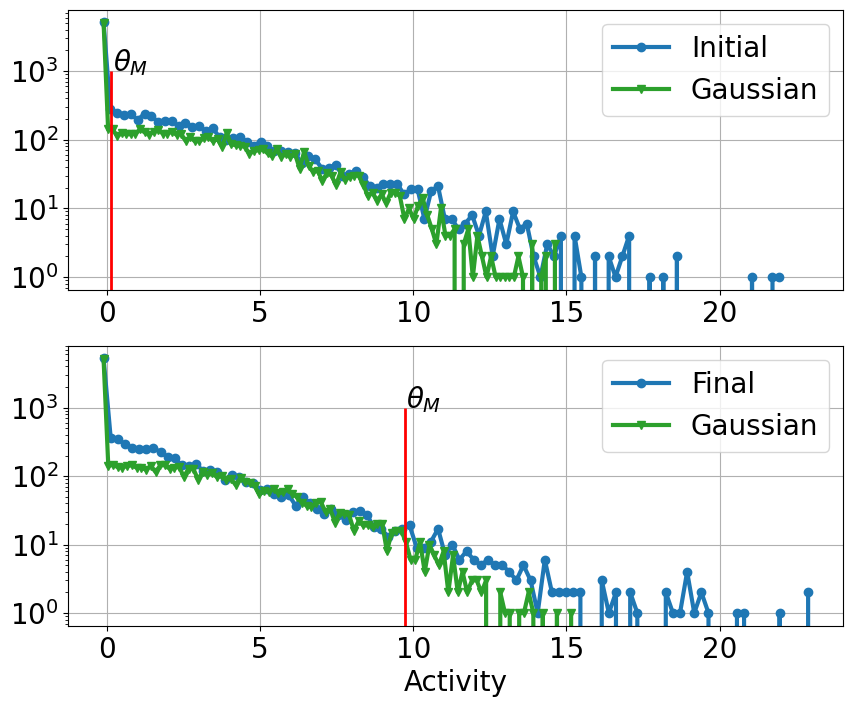
\includegraphics{/Users/bblais/Documents/Git/Amblyopia-Simulation/Manuscript/resources/Pasted image 20240228124702.png}
\caption{Output distributions for a BCM neuron in a 2D Laplace
environment. Shown are (top) the distribution of responses before any
learning and (bottom) after learning compared to a Gaussian distribution
of responses with the same standard deviation. In both cases, the
responses are smeared across the entire range, with fewer patterns
yielding high responses. Because these plots are on a log scale,
Gaussian responses appear curved down as activity increases while
Laplace responses appear as a straight decline. The BCM neuron finds
directions in the input space such that its responses are more Laplacian
-- they respond more to a smaller group of
patterns.}\label{fig:2D_BCM_Laplace}
\end{figure}

\begin{figure}
\centering
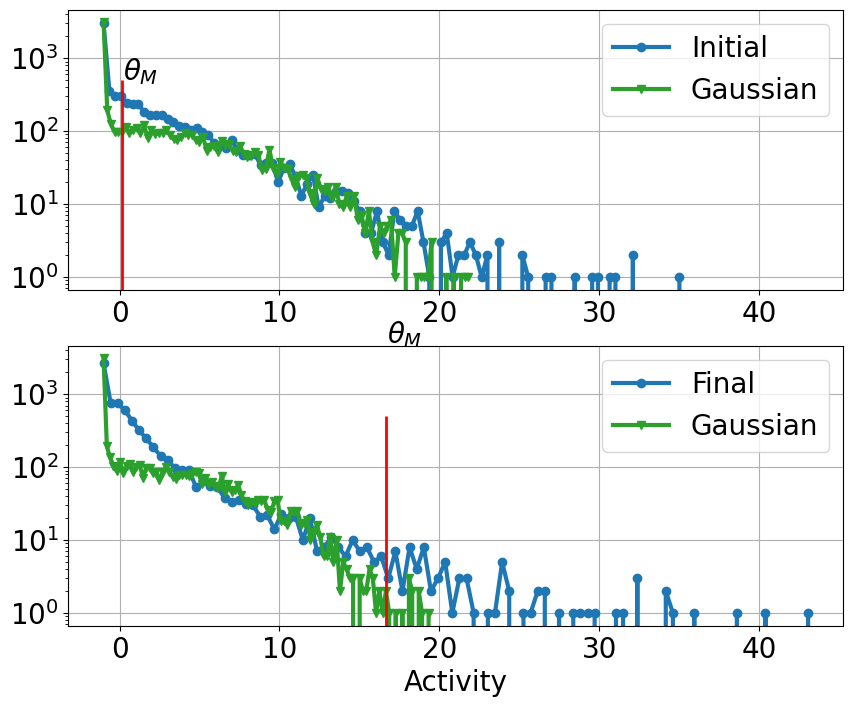
\includegraphics{/Users/bblais/Documents/Git/Amblyopia-Simulation/Manuscript/resources/Pasted image 20240228124932.png}
\caption{Output distributions for a BCM neuron in a natural image
environment. Shown are (top) the distribution of responses before any
learning and (bottom) after learning compared to a Gaussian distribution
of responses with the same standard deviation. In both cases, the
responses are smeared across the entire range, with fewer patterns
yielding high responses. Because these plots are on a log scale,
Gaussian responses appear curved down as activity increases while
Laplace responses appear as a straight decline. The BCM neuron finds
directions in the input space such that its responses are more Laplacian
-- they respond more to a smaller group of
patterns.}\label{fig:BCM_Natural_Image}
\end{figure}

\subsection{Two-eye input
environments}\label{sec:two-eye-input-environments}

Another form of structure occurs with two-eye inputs, where the input
values can be nearly identical -- especially in what we call the
\emph{normal rearing} environment. Examples of this are shown in Figure
\ref{fig:2D_NR}. In the artificial case of completely identical (i.e.~no
input noise, Figure \ref{fig:2D_NR}A), the changes to the left- and
right-eye weights are also identical so the weights can only move along
a parallel 45\(^{\circ}\) line from their starting position. Any
difference between the left- and right-eye weights is preserved as a
result. The added noise (Figure \ref{fig:2D_NR}B) sets up a pattern
competition, where the structure along the input direction dominates
over the noise in the perpendicular direction, and the weights are
driven toward the diagonal. Although the neuron becomes selective in
both cases, the added noise allows for better selectivity and equality
between the left- and right-eye inputs. As is typical with BCM, the
larger the noise the faster the weights are driven toward the structure.

\begin{figure}
\centering
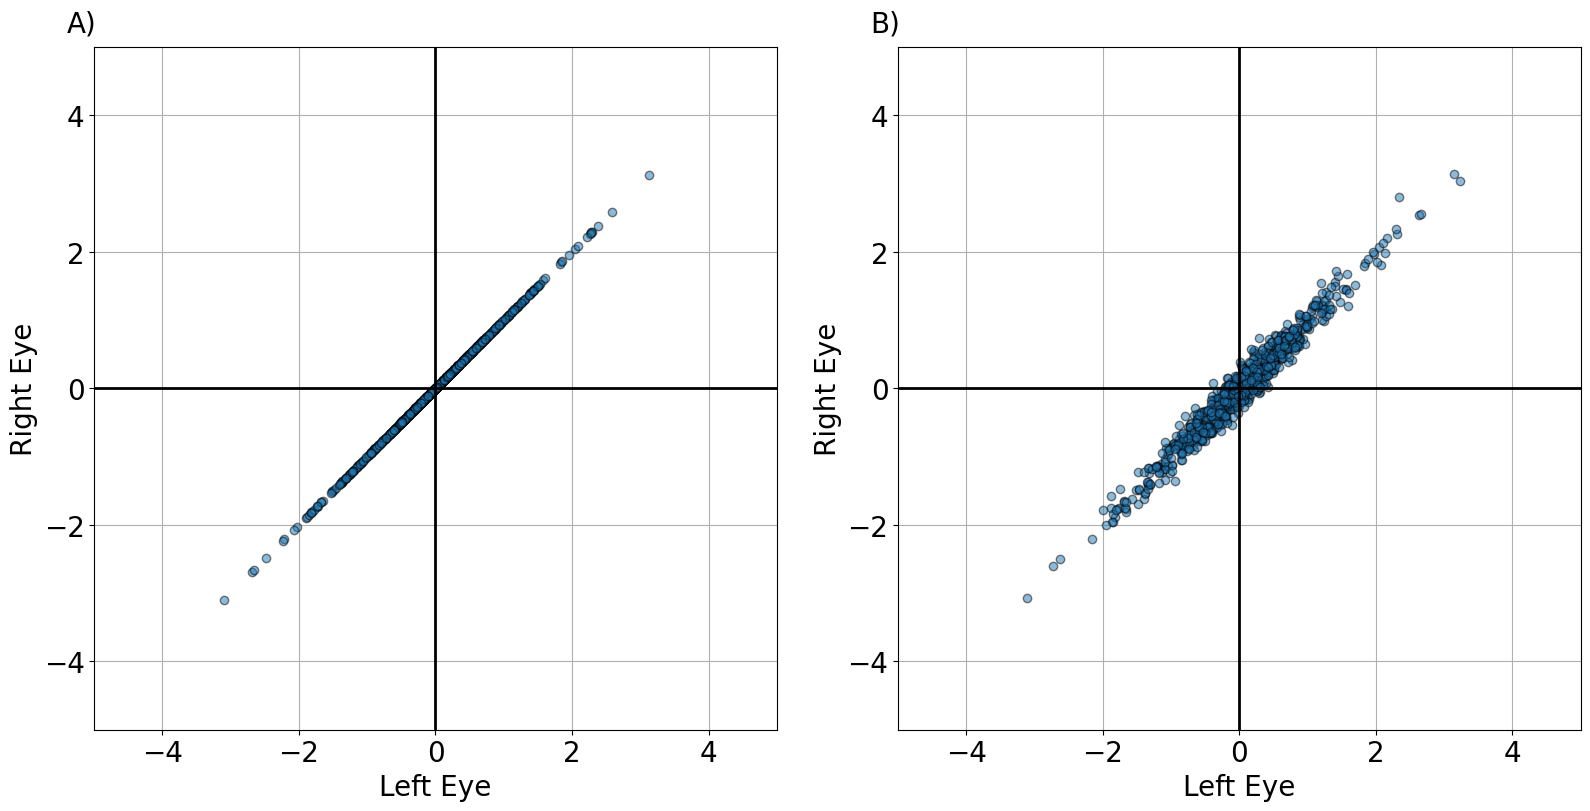
\includegraphics{/Users/bblais/Documents/Git/Amblyopia-Simulation/Manuscript/resources/Pasted image 20240601134351.png}
\caption{2D Normal Rearing inputs where the left- and right-eye inputs
are identical (A) or nearly identical, but differ with normally
distributed noise (B) .}\label{fig:2D_NR_inputs}
\end{figure}

\begin{figure}
\centering
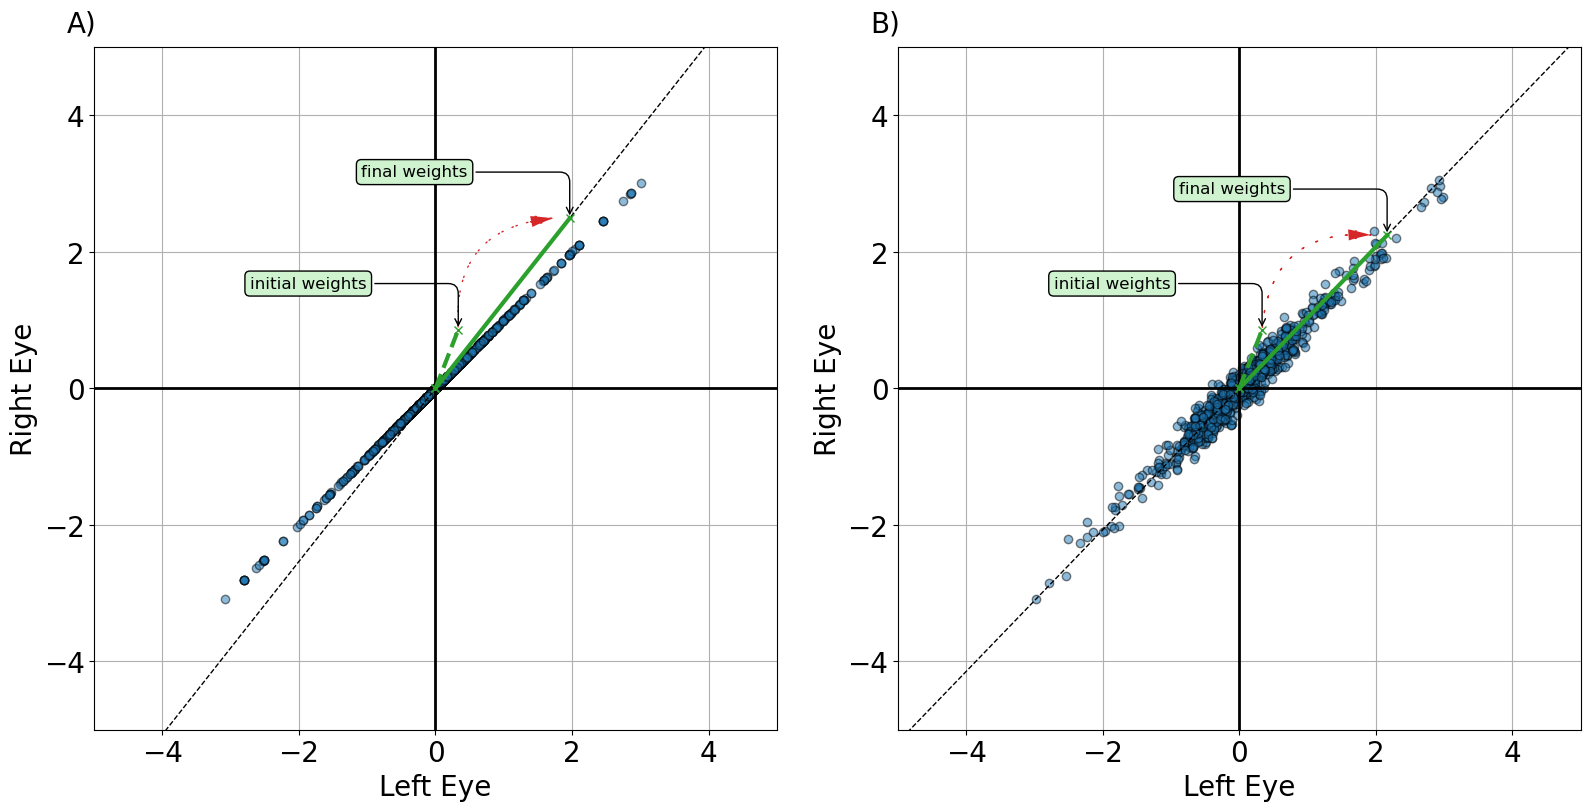
\includegraphics{/Users/bblais/Documents/Git/Amblyopia-Simulation/Manuscript/resources/Pasted image 20240602100107.png}
\caption{BCM in a 2D Normal Rearing environment where the left- and
right-eye inputs are identical (A) or nearly identical, but differ with
normally distributed noise (B). . In the case with identical inputs (A),
the changes to the left- and right-eye weights are also identical so the
weights can only move along a parallel 45\(^{\circ}\) line from their
starting position. The added noise (B) sets up a pattern competition,
where the structure along the input direction dominates over the
perpendicular direction, and the weights are driven toward the
diagonal.}\label{fig:2D_NR_weights}
\end{figure}

The structure vs noise competition occurs even when the noise magnitude
is \emph{larger} than the noise magnitude, Figure
\ref{fig:2D_NR_high_noise}.

\begin{figure}
\centering
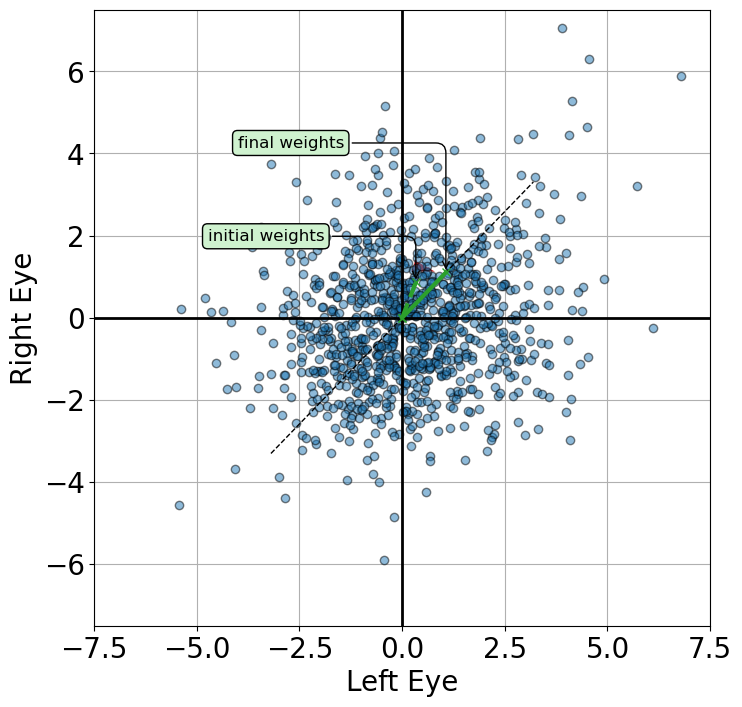
\includegraphics{/Users/bblais/Documents/Git/Amblyopia-Simulation/Manuscript/resources/Pasted image 20240603065355.png}
\caption{The same scenario as shown in Figure \ref{fig:2D_NR_weights}B
but with a noise higher in magnitude than the structure, to the point
that by eye one can't even see the structure but the BCM neuron still
converges to the same direction as maximum
structure.}\label{fig:2D_NR_high_noise}
\end{figure}

\subsubsection{Deprivation}\label{sec:deprivation}

In various deprivation situations we have a sequence where the neuron is
allowed to train in a normal environment and then the environment
switches such that the structure is changed in one or both eye-inputs.
Common deprivation scenarios include the following:

\begin{itemize}
\tightlist
\item
  Monocular deprivation: (structure,structure) \(\rightarrow\)
  (noise,structure)
\item
  Binocular deprivation: (structure,structure) \(\rightarrow\)
  (noise,noise)
\item
  Contrast deprivation: (structure,structure) \(\rightarrow\) (structure
  \(\times\) contrast factor,structure)
\item
  Reverse occlusion: (structure,structure) \(\rightarrow\)
  (noise,structure) \(\rightarrow\) (structure,noise)
\item
  Binocular recovery: (structure,structure) \(\rightarrow\)
  (noise,structure) \(\rightarrow\) (structure,structure)
\end{itemize}

The first three (monocular deprivation,binocular deprivation, and
contrast deprivation) are shown in Figure \ref{fig:NR_MD_BD_CD}.

\begin{figure}
\centering
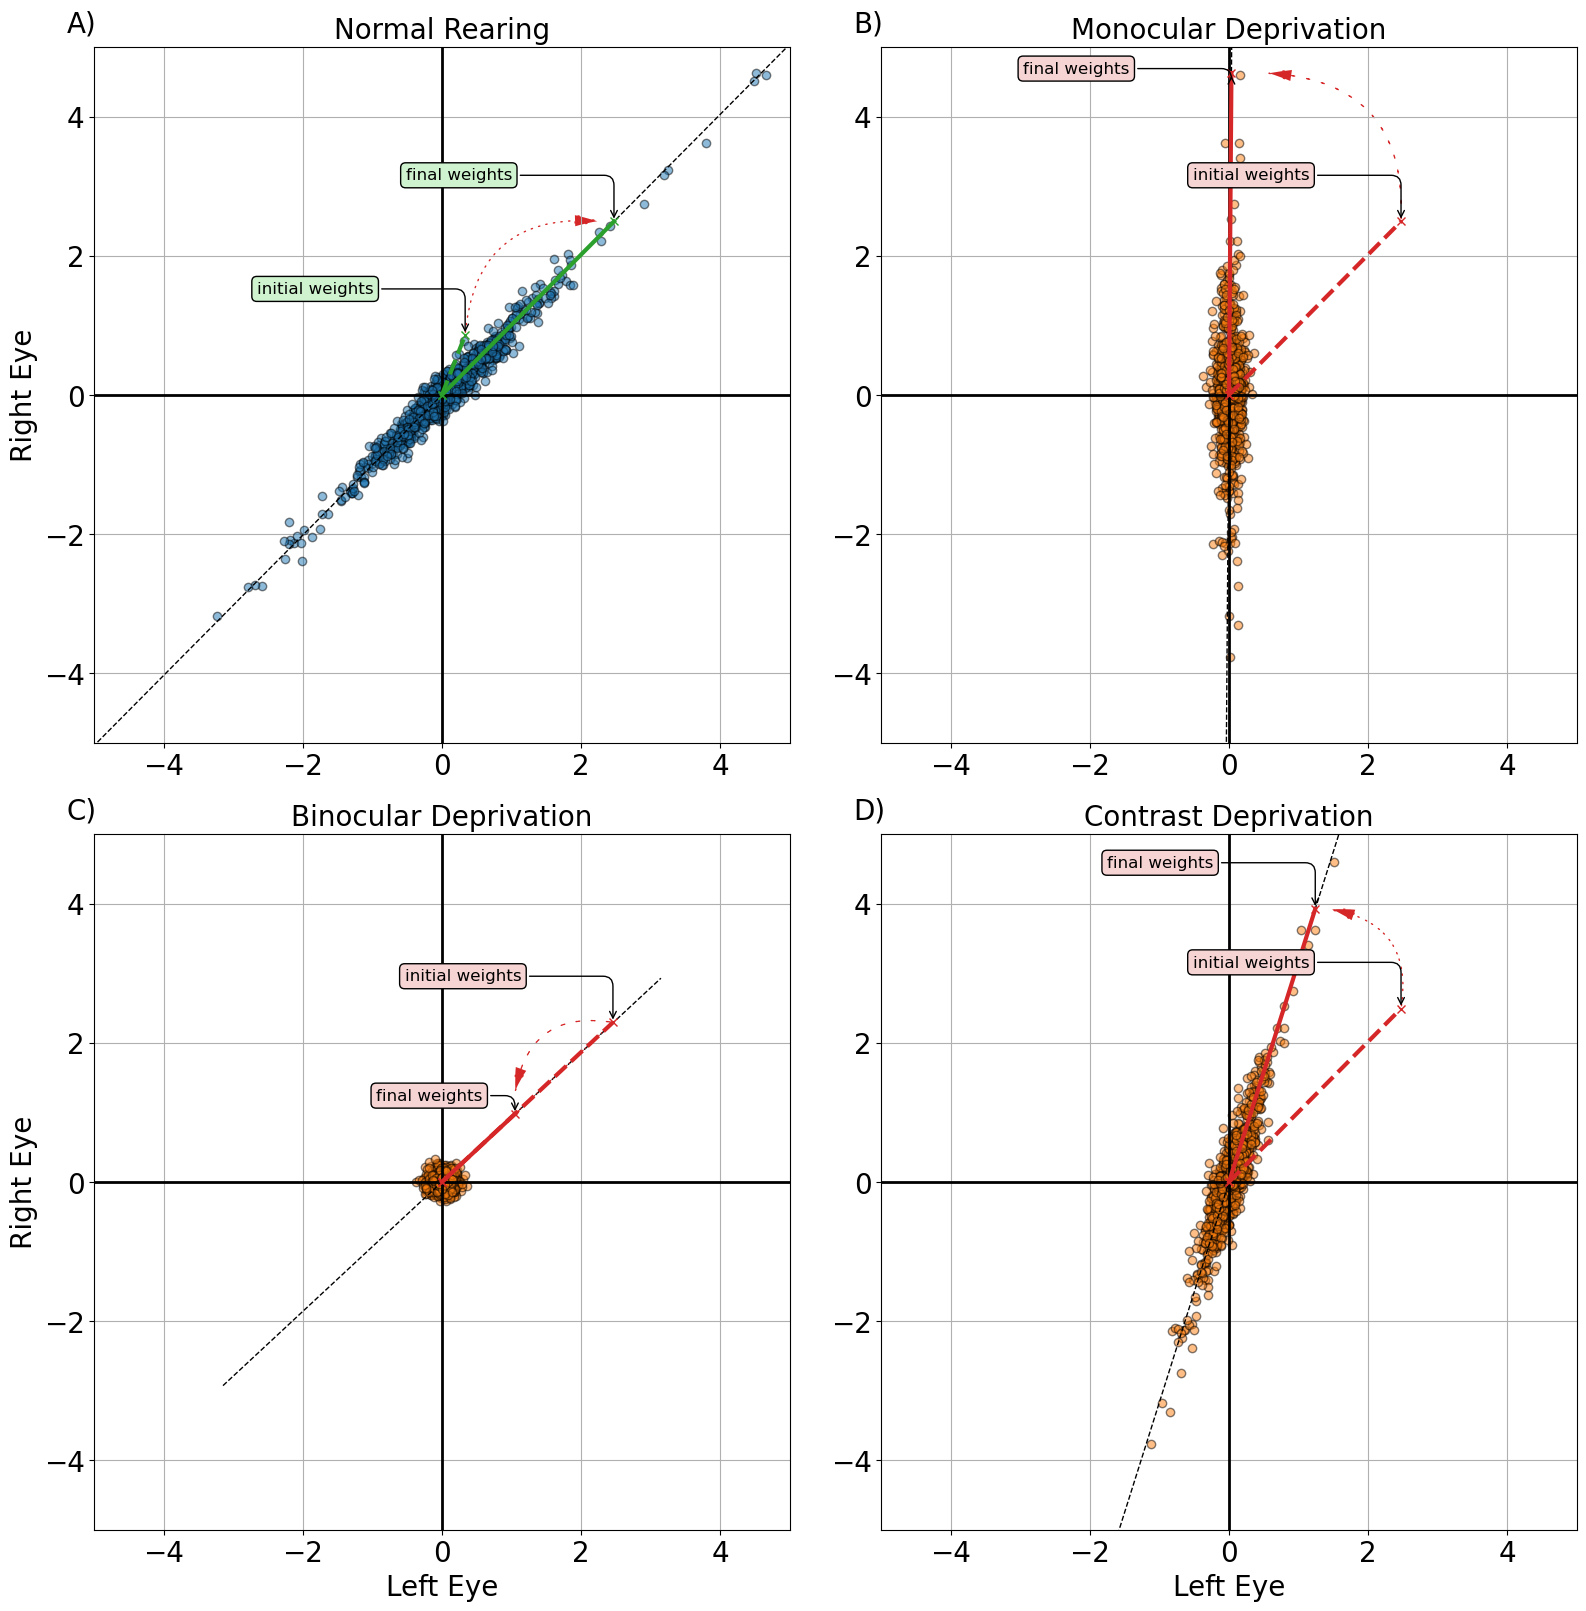
\includegraphics{/Users/bblais/Documents/Git/Amblyopia-Simulation/Manuscript/resources/Pasted image 20240602095046.png}
\caption{BCM under conditions of normal rearing (A), monocular
deprivation (B), binocular deprivation (C), and contrast deprivation (D)
in a 2D environment. In each case the weights are driven toward the
direction of largest
structure.}\label{fig:Pasted_image_20240602095046.png}
\end{figure}

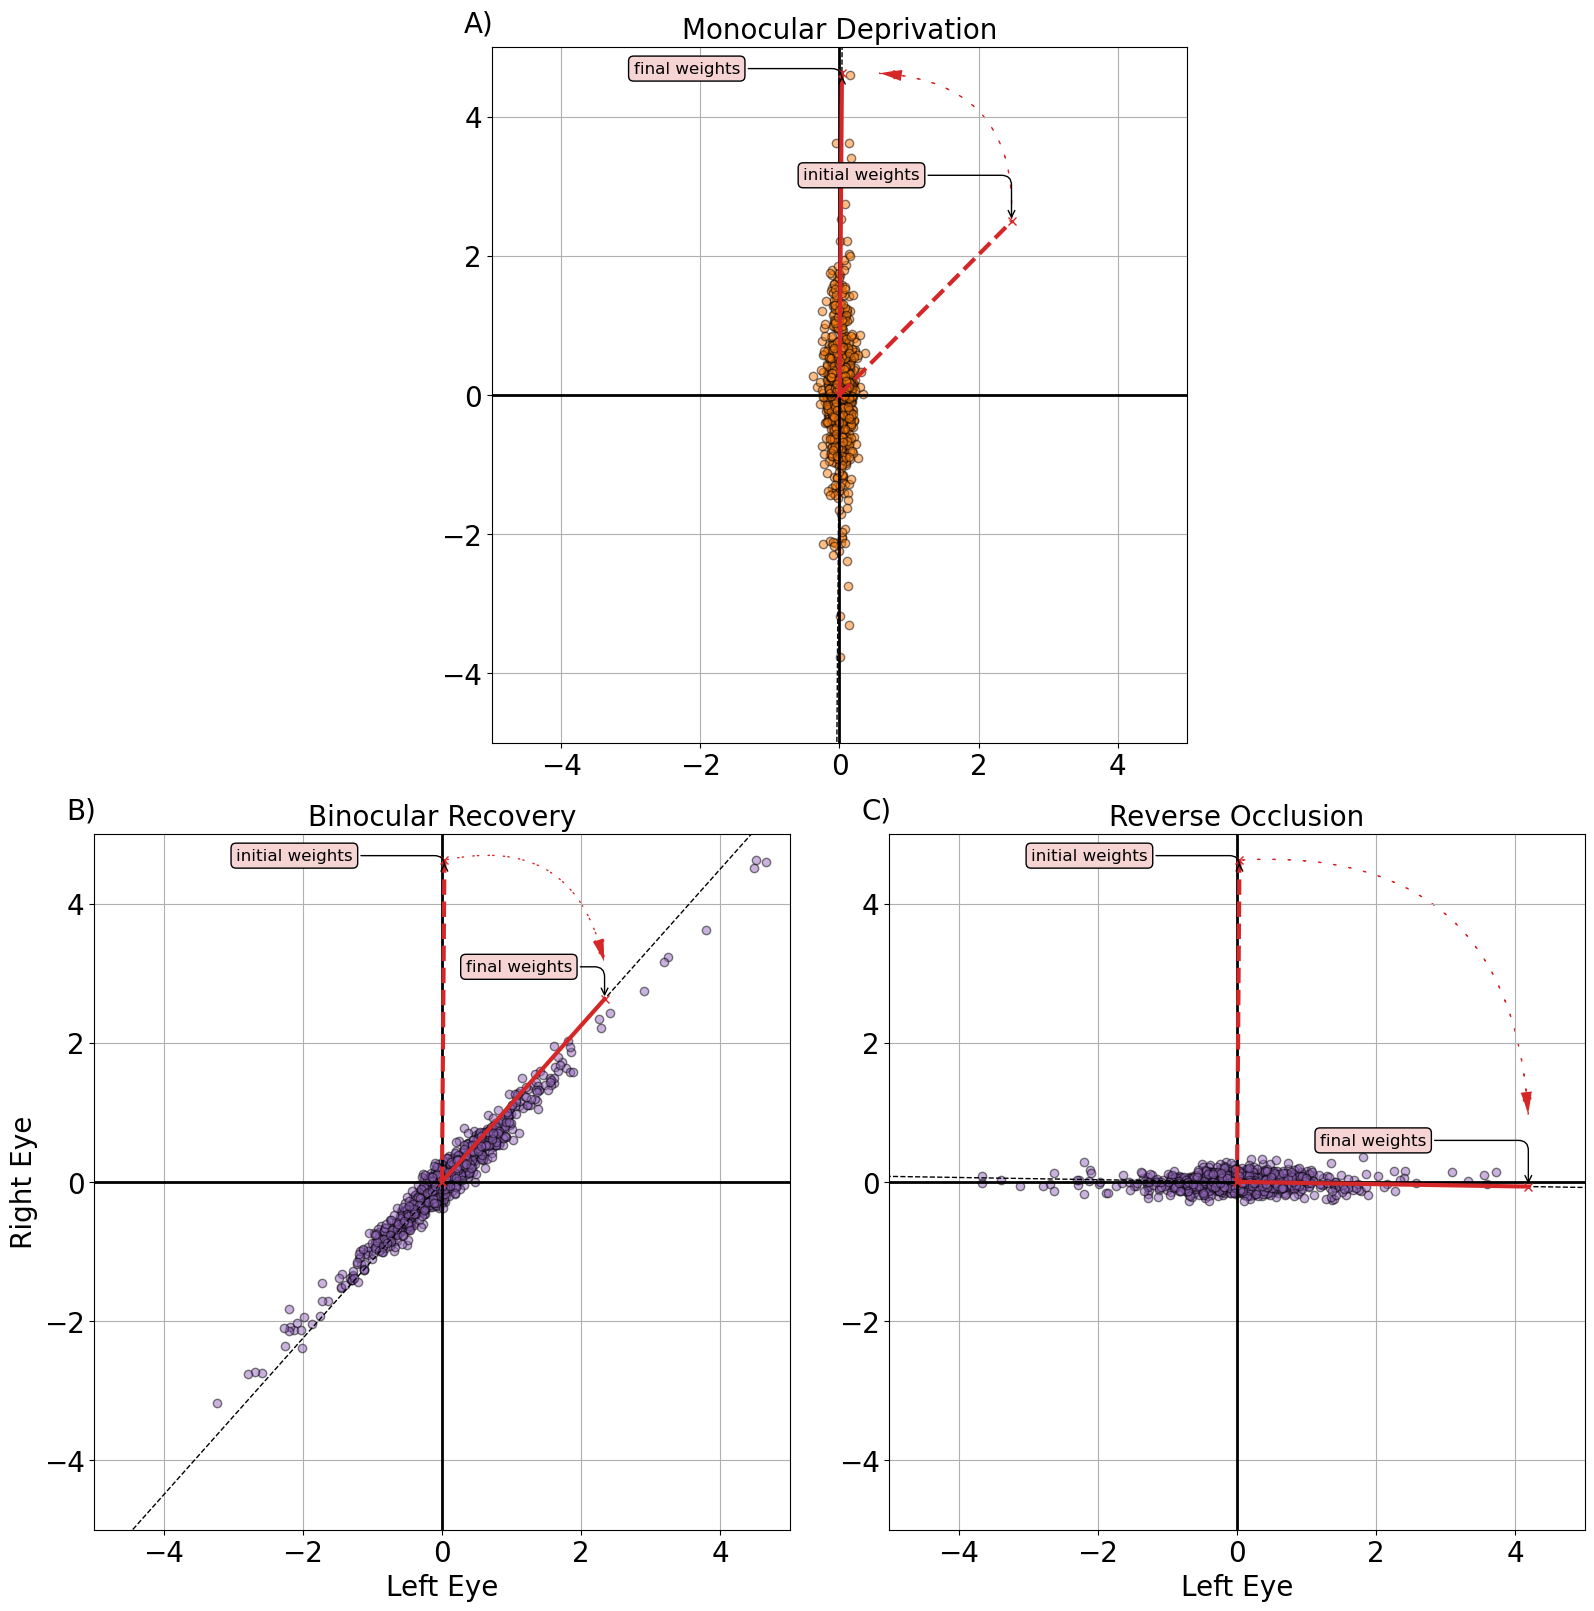
\includegraphics{/Users/bblais/Documents/Git/Amblyopia-Simulation/Manuscript/resources/Pasted image 20240602095113.png}\{\#figref:Pasted
image 20240602095113.png\}

\#todo - {[} {]} talk about MD, BD, RS, and BR

\section{Normal and Deprived Visual
Environments}\label{sec:normal-and-deprived-visual-environments}

In order to approximate the visual system, we start with the following
basic properties of the retina, LGN and cortex. There are approximately
1000 photoreceptors feeding into 1 ganglion cell\textsuperscript{7,8}.
The retina/LGN responses show a center-surround organization, but with a
center diameter less than 1\(^o\)\textsuperscript{9}

We use natural scene stimuli for the simulated inputs to the visual
system. We start with images taken with a digital camera, with
dimensions 1200 pixels by 1600 pixels and 40\(^o\) by 60\(^o\)
real-world angular dimensions (Figure \ref{fig:natural_images}). We
model the light adaption of the photoreceptors\textsuperscript{10,11}
where the responses reflect the contrast (i.e.~difference from the mean,
\(I_m\)) and normalized to the standard deviation of the pixel values,
\(I_\sigma\),

\[
R=\frac{I-I_m}{I_\sigma}
\] Finally, we model the contrast normalization and the suppressive
field of the ganglion responses using a 32x32 pixel center-surround
difference-of-Gaussians (DOG) filter to process the images (Figure
\ref{fig:normal_vision_model}). The center-surround radius ratio used
for the ganglion cell is 1:3, with balanced excitatory and inhibitory
regions and normalized Gaussian profiles. Even in the normal visual
environment we explore the role of eye-jitter, where the locations of
the left- and right-receptive fields are chosen to deviate from a common
center by an average shift, \(\mu_c\), and variation, \(\sigma_c\) (see
Figure \ref{fig:eye_jitter}).

\begin{figure}
\centering
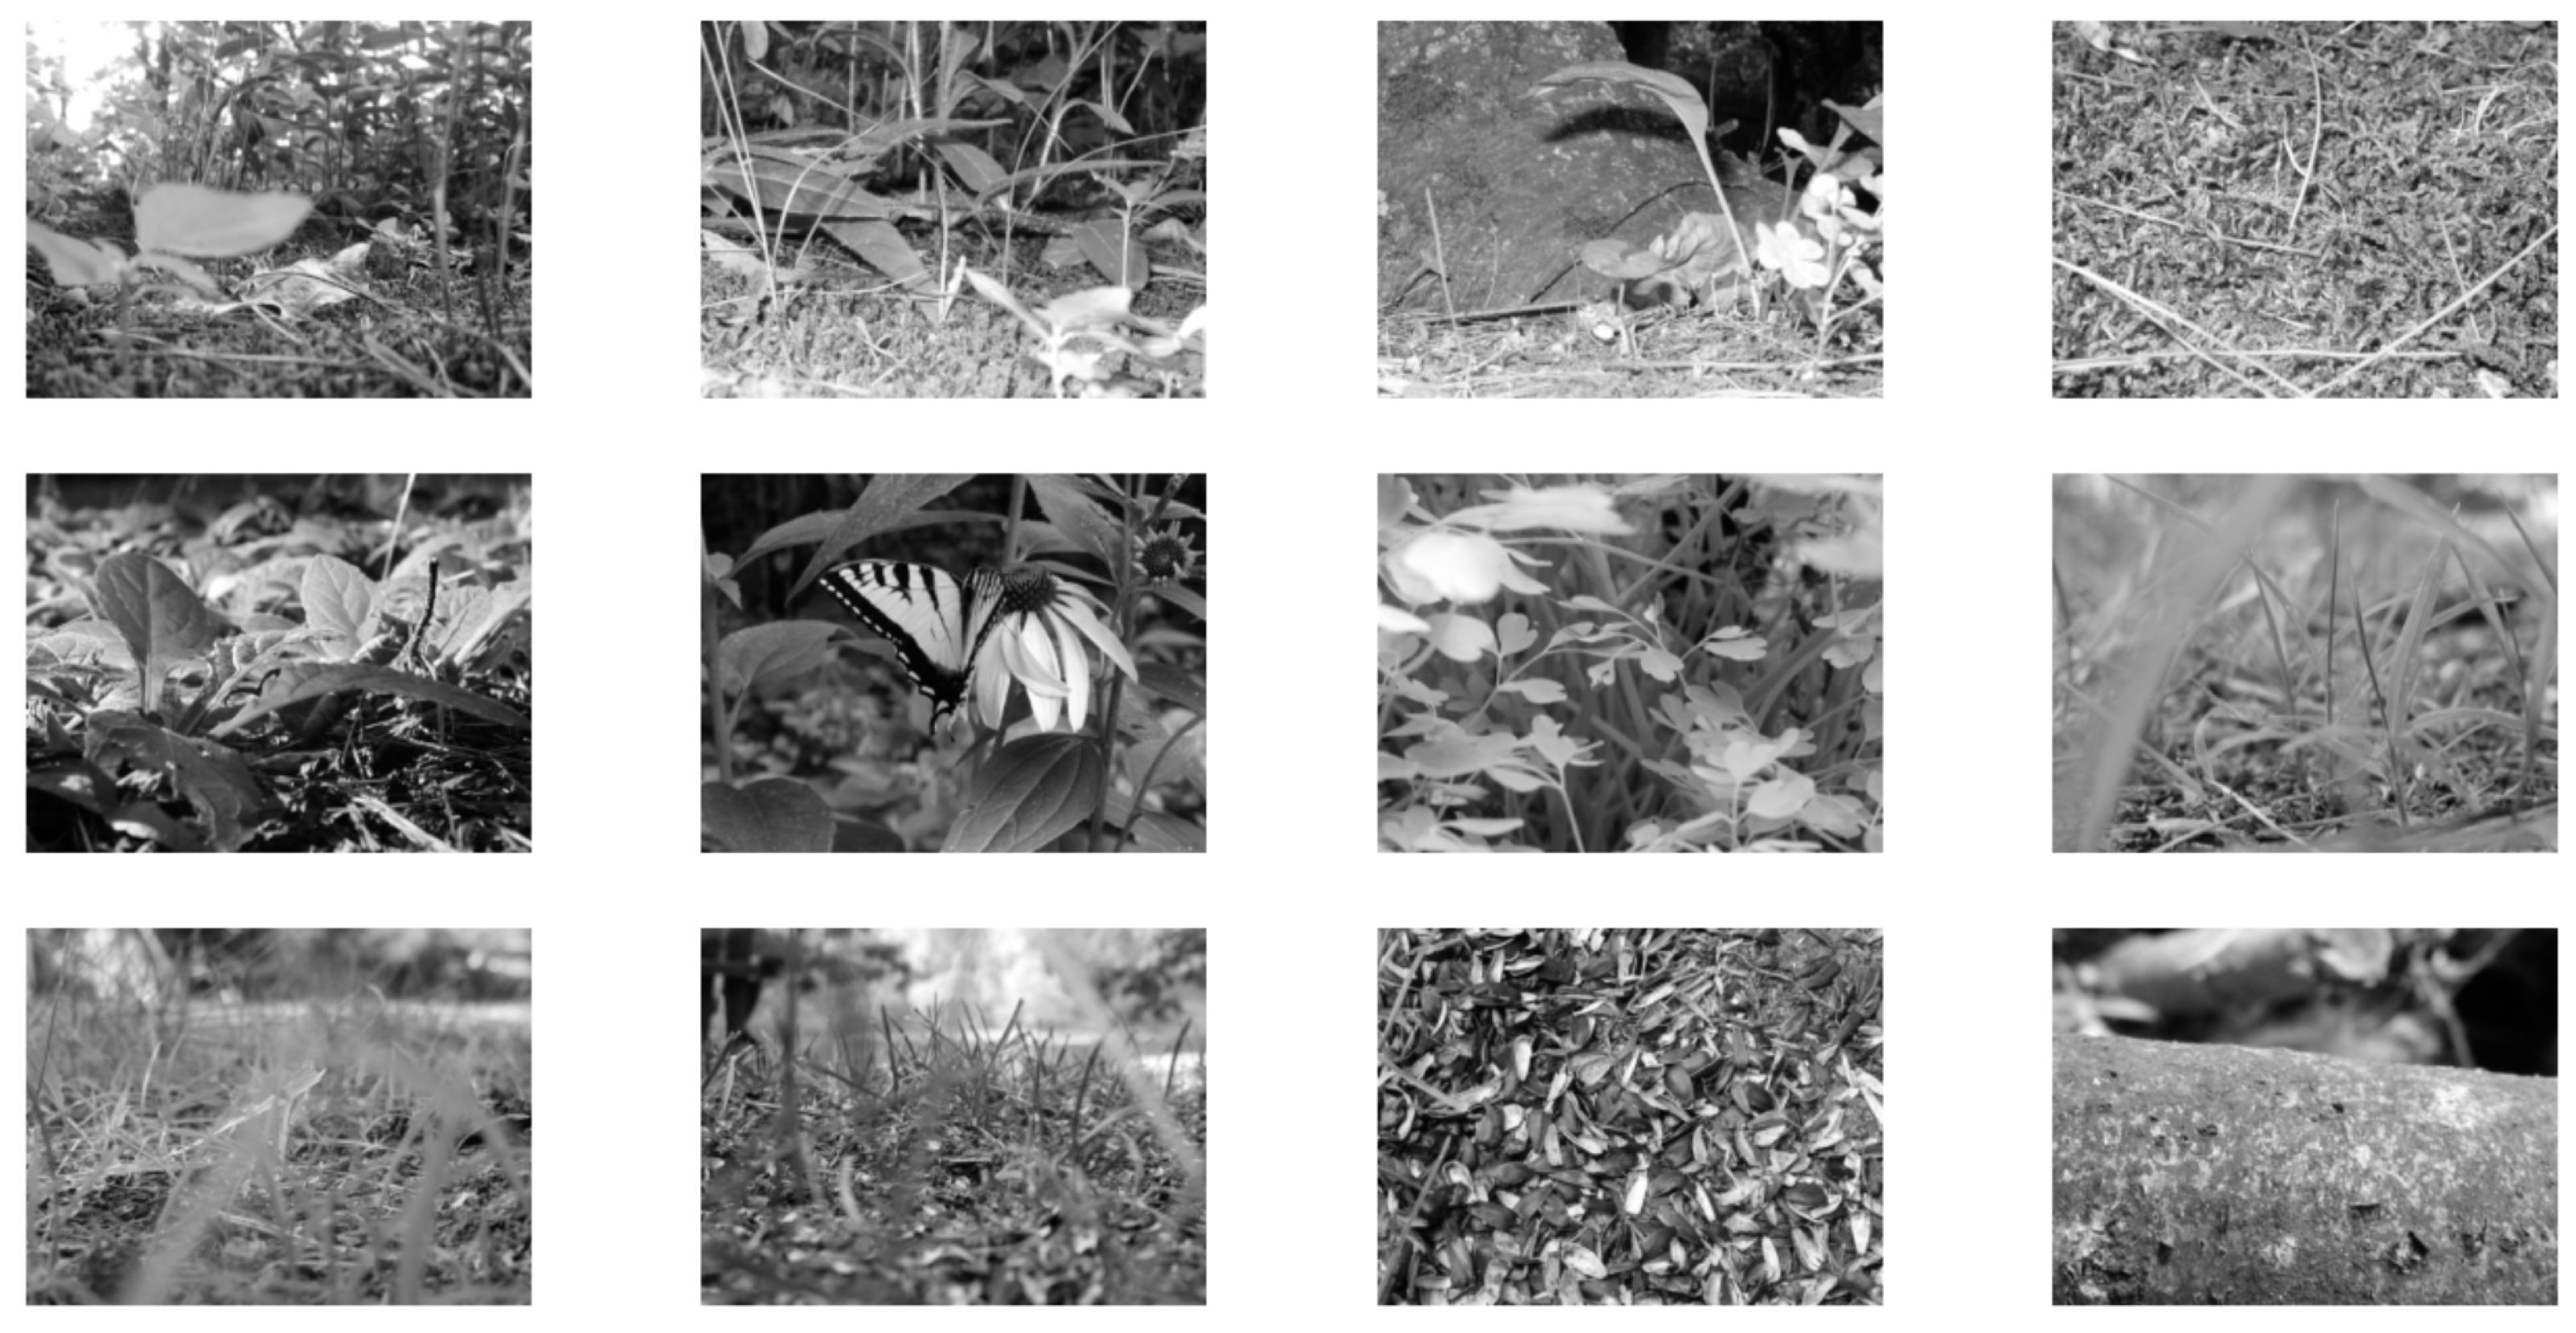
\includegraphics{/Users/bblais/Documents/Git/Amblyopia-Simulation/Manuscript/resources/Pasted image 20240301091111.png}
\caption{Natural Image Environment.}\label{fig:natural_images}
\end{figure}

\begin{figure}
\centering
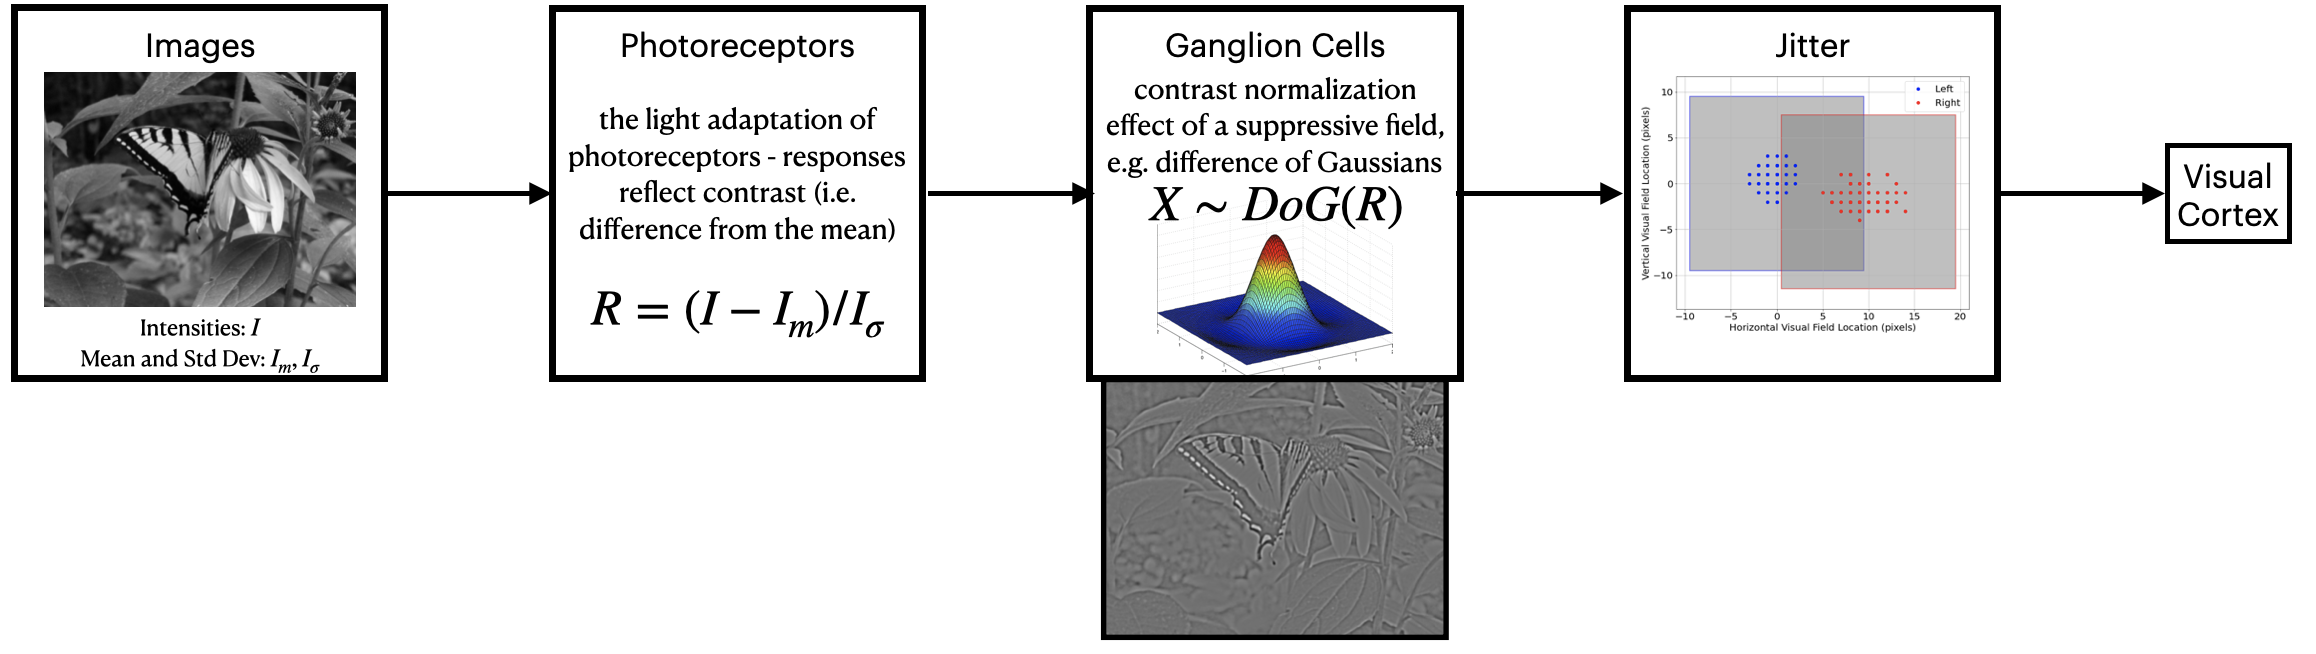
\includegraphics{/Users/bblais/Documents/Git/Amblyopia-Simulation/Manuscript/resources/Pasted image 20240301091213.png}
\caption{Normal Vision Model.}\label{fig:normal_vision_model}
\end{figure}

\begin{figure}
\centering
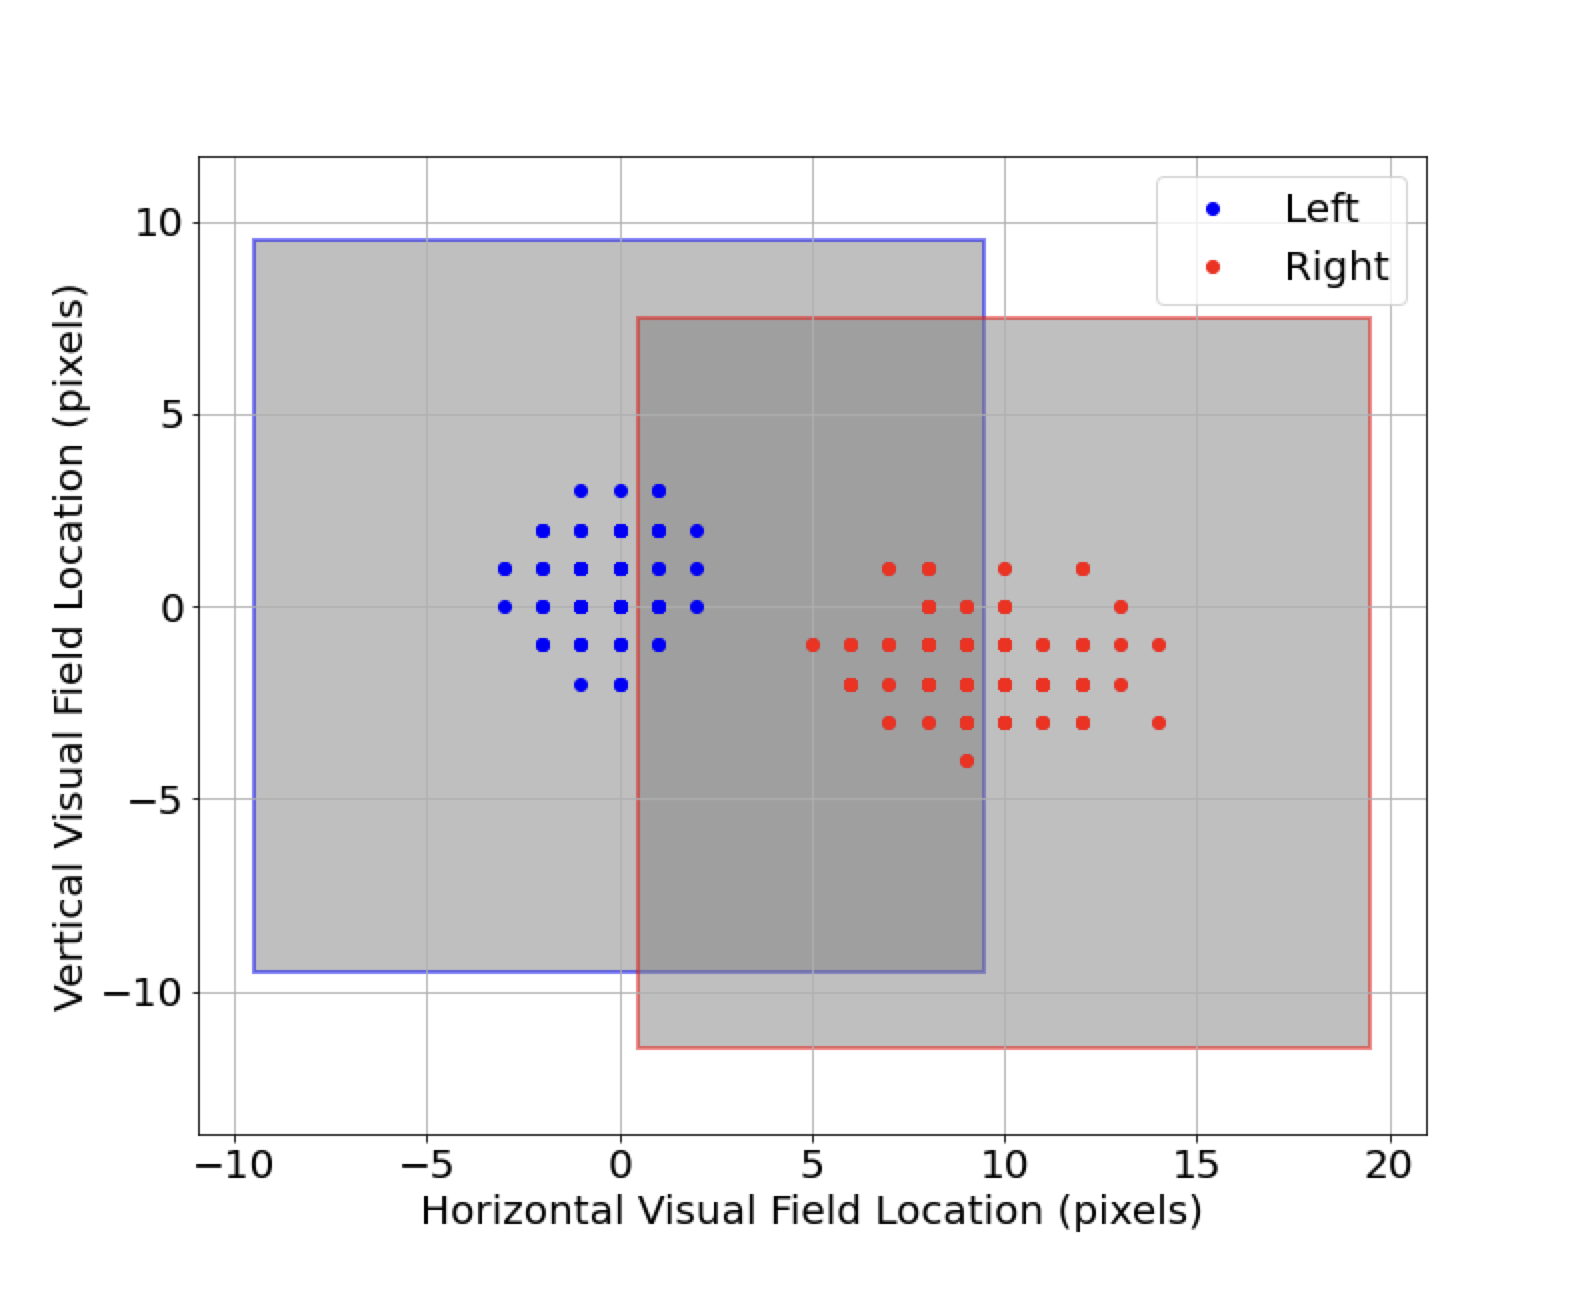
\includegraphics{/Users/bblais/Documents/Git/Amblyopia-Simulation/Manuscript/resources/Pasted image 20240301091231.png}
\caption{Model of Eye Jitter.}\label{fig:eye_jitter}
\end{figure}

\subsubsection{Two-eye architecture}\label{sec:two-eye-architecture}

Shown in Figure \ref{fig:arch} is the visual field, approximated here as
a two-dimensional projection, to left and right retinal cells. These
left and right retinal cells project to the left and right LGN cells,
respectively, and finally to a single cortical cell. The LGN is assumed
to be a simple relay, and does not modify the incoming retinal activity.
It is important to understand that the model we are pursuing here is a
\emph{single cortical cell} which receives input from both eyes. We will
encounter some limitations to this model which may necessitate exploring
multi-neuron systems.

In the model, normal development is simulated with identical image
patches presented to both eyes combined with small independent noise in
each eye. The random noise is generated from a zero-mean normal
distribution of a particular variance, representing the natural
variation in responses of LGN neurons. Practically, the independent
random noise added to each of the two-eye channels avoids the artificial
situation of having mathematically identical inputs in the channels. The
development of the deficit and the subsequent treatment protocols are
modeled with added preprocessing to these image patches, described below
in Section
sec.~\ref{sec:models-of-development-and-treatment-of-amblyopia}.

For all of the simulations we use a 19x19 receptive field, which is a
compromise between speed of simulation and the limits of spatial
discretization. We perform at least 20 independent simulations for each
condition to address variation in the results.

\begin{figure}
\centering
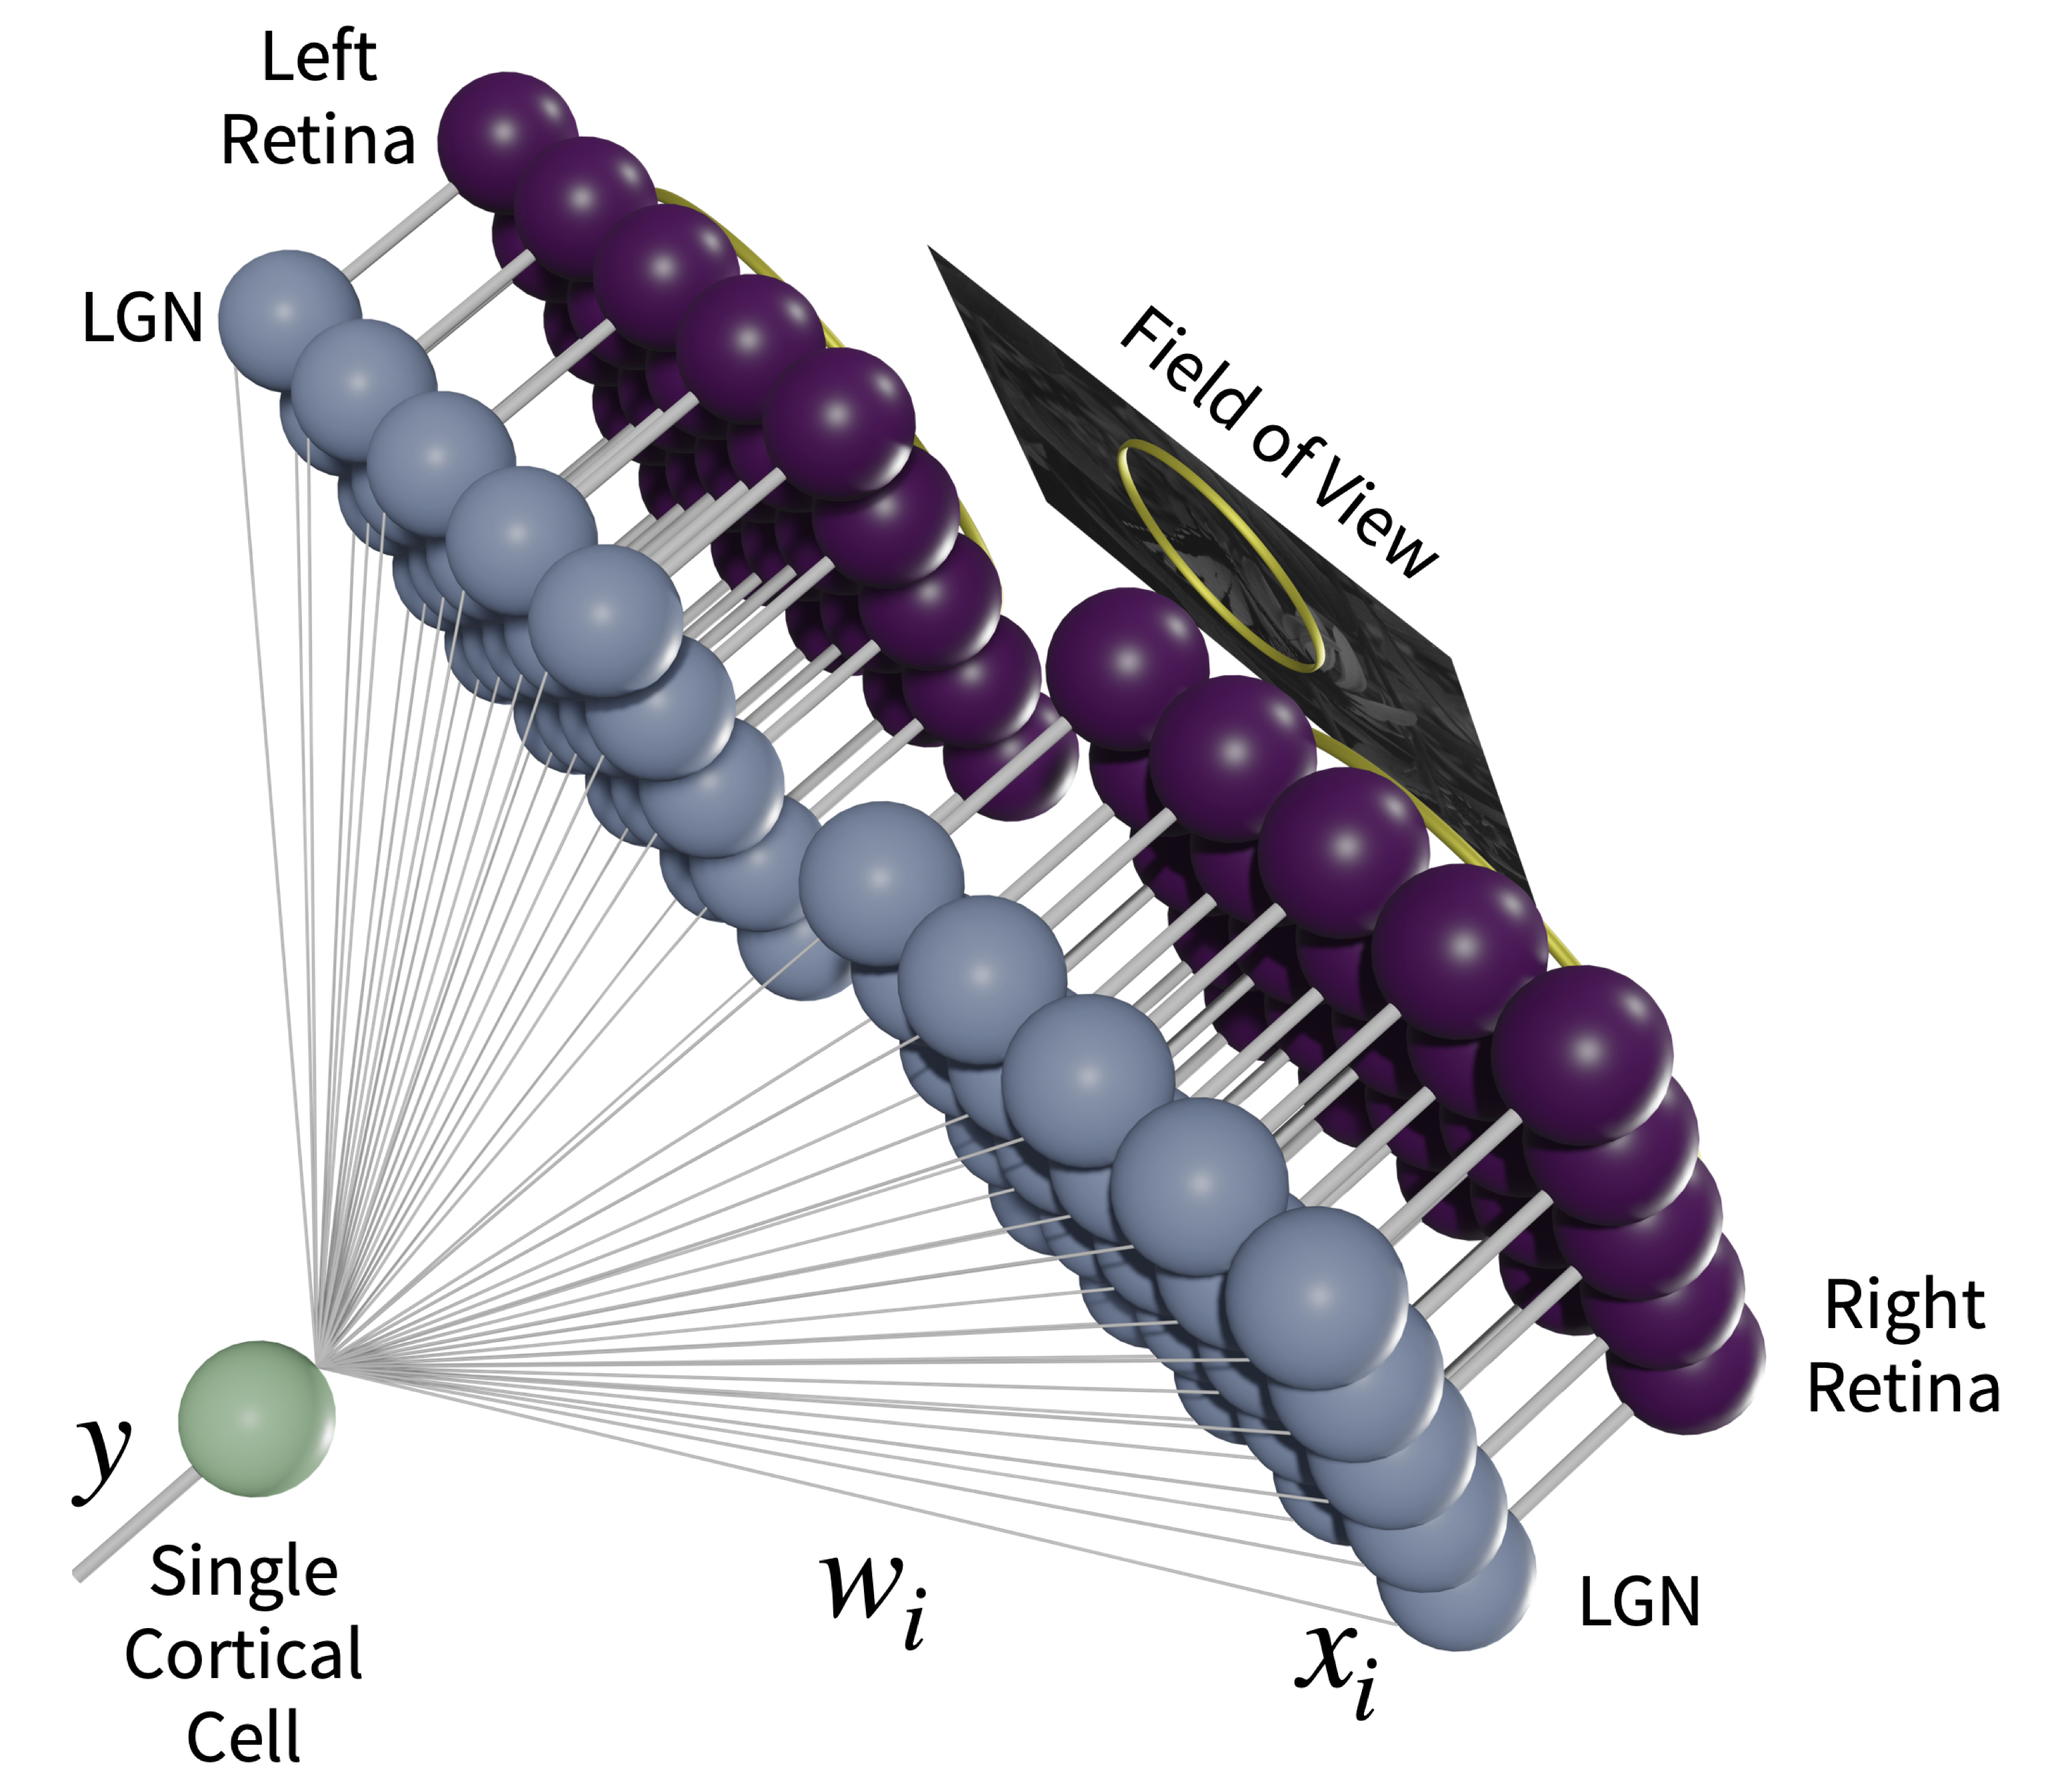
\includegraphics{/Users/bblais/Documents/Git/Amblyopia-Simulation/Manuscript/resources/Pasted image 20240301091247.png}
\caption{Architecture for binocular neurons in natural image
environment.}\label{fig:arch}
\end{figure}

\subsection{Ocular Dominance Index}\label{sec:ocular-dominance-index}

Simulations are ended when selectivity has been achieved and the
responses are stable. From the maximal responses of each eye,
\(R_{\text{left}}\) and \(R_{\text{right}}\), individually, we can
calculate the ocular dominance index as \[
\text{ODI} \equiv \frac{R_{\text{right}}-R_{\text{left}}}{R_{\text{right}}+R_{\text{left}}}
\] The ocular dominance index (ODI) has a value of
\(\text{ODI} \approx 1\) when stimulus to the right-eye (typically the
fellow-eye in the simulations, by convention) yields a maximum neuronal
response with little or no contribution from the left-eye. Likewise, an
ocular dominance index (ODI) has a value of \(\text{ODI} \approx -1\)
when stimulus to the left-eye (typically the amblyopic-eye, by
convention) yields a maximum neuronal response with little or no
contribution from the right-eye. A value of \(\text{ODI} \approx 0\)
represents a purely binocular cell, responding equally to stimulus in
either eye.

Recovery and deprivation speed is measured in ODI shift over the time of
simulation, with the units of time are arbitrary. This allows us to
compare different treatment protocols and examine how the rates of
deprivation vary based on the simulation and environment parameters.

\subsection{Models of Deprivation}\label{sec:models-of-deprivation}

\subsection{Models of Development and Treatment of
Amblyopia}\label{sec:models-of-development-and-treatment-of-amblyopia}

Here we explore the model environments for the initial deficit and the
treatments. Amblyopia is achieved by an imbalance in right and left
inputs, and treated with a re-balance or a counter-balance of those
inputs (e.g.~patching the dominant eye). In this work, we model the
initial deficit as resulting from an asymmetric \emph{blurring} of the
visual inputs, as would be produced by a refractive difference between
the eyes ({[}Figure fig:vision\_deficit\_model{]}). The amblyopic eye is
presented with image patches that have been \emph{blurred} with a
normalized Gaussian filter applied to the images with a specified width.
The larger the width the blurrier the resulting filtered image. Using a
blur filter size of 2.5 pixels produces a robust deficit in the
simulations, and thus we use this deficit as the starting point for all
of the treatment simulations. Although both eyes receive nearly
identical input patches, we add independent Gaussian noise to each input
channel to represent the natural variation in the activity in each eye.

In addition to the refractive deficit we also model a strabismic jitter
in the input pattern, represented as a pixel-shift of the input column
and row with means \(\mu_c\) and \(\mu_r\), respectively, with standard
deviations \(\sigma_c\) and \(\sigma_r\), respectively. For example, in
the simple case of \(\mu_c=\mu_r=0\) and \(\sigma_c=\sigma_r=0\) the eye
inputs are identical (up to intrinsic noise). If \(\mu_c=5\) then the
input images for the two channels are shift left-right by a constant 5
pixels. If \(\mu_c>19\) (with 19 being the receptive field size), then
the eyes will see completely non-overlapping areas of the image.

To model the optical fix to the refractive imbalance we follow the
deficit simulation with an input environment that is rebalanced, both
eyes receiving nearly identical input patches (Figure
\ref{fig:optical_fix_mode}). This process is a model of the application
of glasses. The optical fix will remove the refractive deficit but will
not treat any strabismic jitter.

\subsubsection{Patch treatment}\label{sec:patch-treatment}

The typical patch treatment is done by depriving the fellow-eye of input
with an eye-patch. In the model this is equivalent to presenting the
fellow-eye with random noise instead of the natural image input (Figure
\ref{fig:patch_model}). Competition between the left- and right-channels
drives the recovery, and is produced from the difference between
\emph{structured} input into the amblyopic-eye and the
\emph{unstructured} (i.e.~noise) input into the fellow-eye. It is not
driven by a reduction in input activity. As shown in
sec.~\ref{sec:results}, increased \emph{unstructured} input into the
previously dominant eye increases the rate of recovery. This is a
general property of the BCM learning rule and has been explored in
Section \ref{sec:structure-vs-noise}.

\subsubsection{Atropine treatment}\label{sec:atropine-treatment}

In the atropine treatment for amblyopia\textsuperscript{12}, eye-drops
of atropine are applied to the fellow-eye resulting in blurred vision in
that eye. Here we use the same blurred filter used to obtain the deficit
(possibly with a different width) applied to the fellow eye (Figure
\ref{fig:atropine_model}) along with an additional amount of noise. The
difference in sharpness between the fellow-eye inputs and the
amblyopic-eye inputs sets up competition between the two channels with
the advantage given to the amblyopic-eye.

\subsubsection{Contrast modification}\label{sec:contrast-modification}

A binocular approach to treatment can be produced with contrast
reduction of the non-deprived channel relative to the deprived channel.
Experimentally this can be accomplished with VR
headsets\textsuperscript{13}. In the model we implement this by
transforming the image toward the average proportional to a simple
scalar contrast value, \[
I_{\text{new}} = I_{\text{orig}} \cdot \text{constrast} + I_m\cdot(1-\text{contrast})
\] where \(I_m\) is an image consisting of a single uniform gray value
of the average of the original image, \(I_{\text{orig}}\). When
\(\text{constrast}=1\) there is no transformation, whereas a value of
\(\text{constrast}=0\) results in the image replaced with a uniform gray
value of the mean image, \(I_m\) (Figure \ref{fig:contrast_mask_model}).
The contrast difference sets up competition between the two channels
with the advantage given to the amblyopic-eye channel.

\subsubsection{Dichoptic Mask}\label{sec:dichoptic-mask}

On top of the contrast modification, we can include the application of
the dichoptic mask (Figure \ref{fig:contrast_mask_model}). In this
method, each eye receives a version of the input images filtered through
independent masks in each channel, resulting in a mostly-independent
pattern in each channel. It has been observed that contrast modification
combined with dichoptic masks can be an effective treatment for
amblyopia\textsuperscript{15}. The motivation behind the application of
the mask filter is that the neural system must use both channels to
reconstruct the full image and thus may lead to enhanced recovery.

The dichoptic masks are constructed with the following procedure. A
blank image (i.e.~all zeros) is made to which is added 15 randomly sized
circles with values equal to 1 (Figure \ref{fig:dichopic_blob}). These
images are then smoothed with a Gaussian filter of a given width, \(f\).
This width is a parameter we can vary to change the overlap between the
left- and right-eye images. A high value of \(f\) compared with the size
of the receptive field, e.g.~\(f=90\), yields a high overlap between the
patterns in the amblyopic- and fellow-eye inputs (Figure
\ref{fig:dichopic_filter_size}). Likewise, a small value of \(f\),
e.g.~\(f=10\), the eye inputs are nearly independent -- the patterned
activity falling mostly on one of the eyes and not much to both.
Finally, the smoothed images are scaled to have values from a minimum of
0 to a maximum of 1. This image-mask we will call \(A\), and is applied
to left-eye whereas the right-eye mask, \(F\), is the inverse of the
left-eye mask, \(F\equiv 1-A\). The mask is applied to an image by
weighting original image and the uniform gray value average, \(I_m\), by
the strength of the mask. ,

\[
\begin{aligned}
I_{\text{left}} &= I_{\text{orig}} \cdot A + I_m\cdot(1-A) \\
I_{\text{right}} &= I_{\text{orig}} \cdot F + I_m\cdot(1-F)
\end{aligned}
\] resulting in a pair of images which have no overlap at the peaks of
each mask, and nearly equal overlap in the areas of the images where the
masks are near 0.5 (Figure \ref{fig:dichopic_filter_image}).

\begin{figure}
\centering
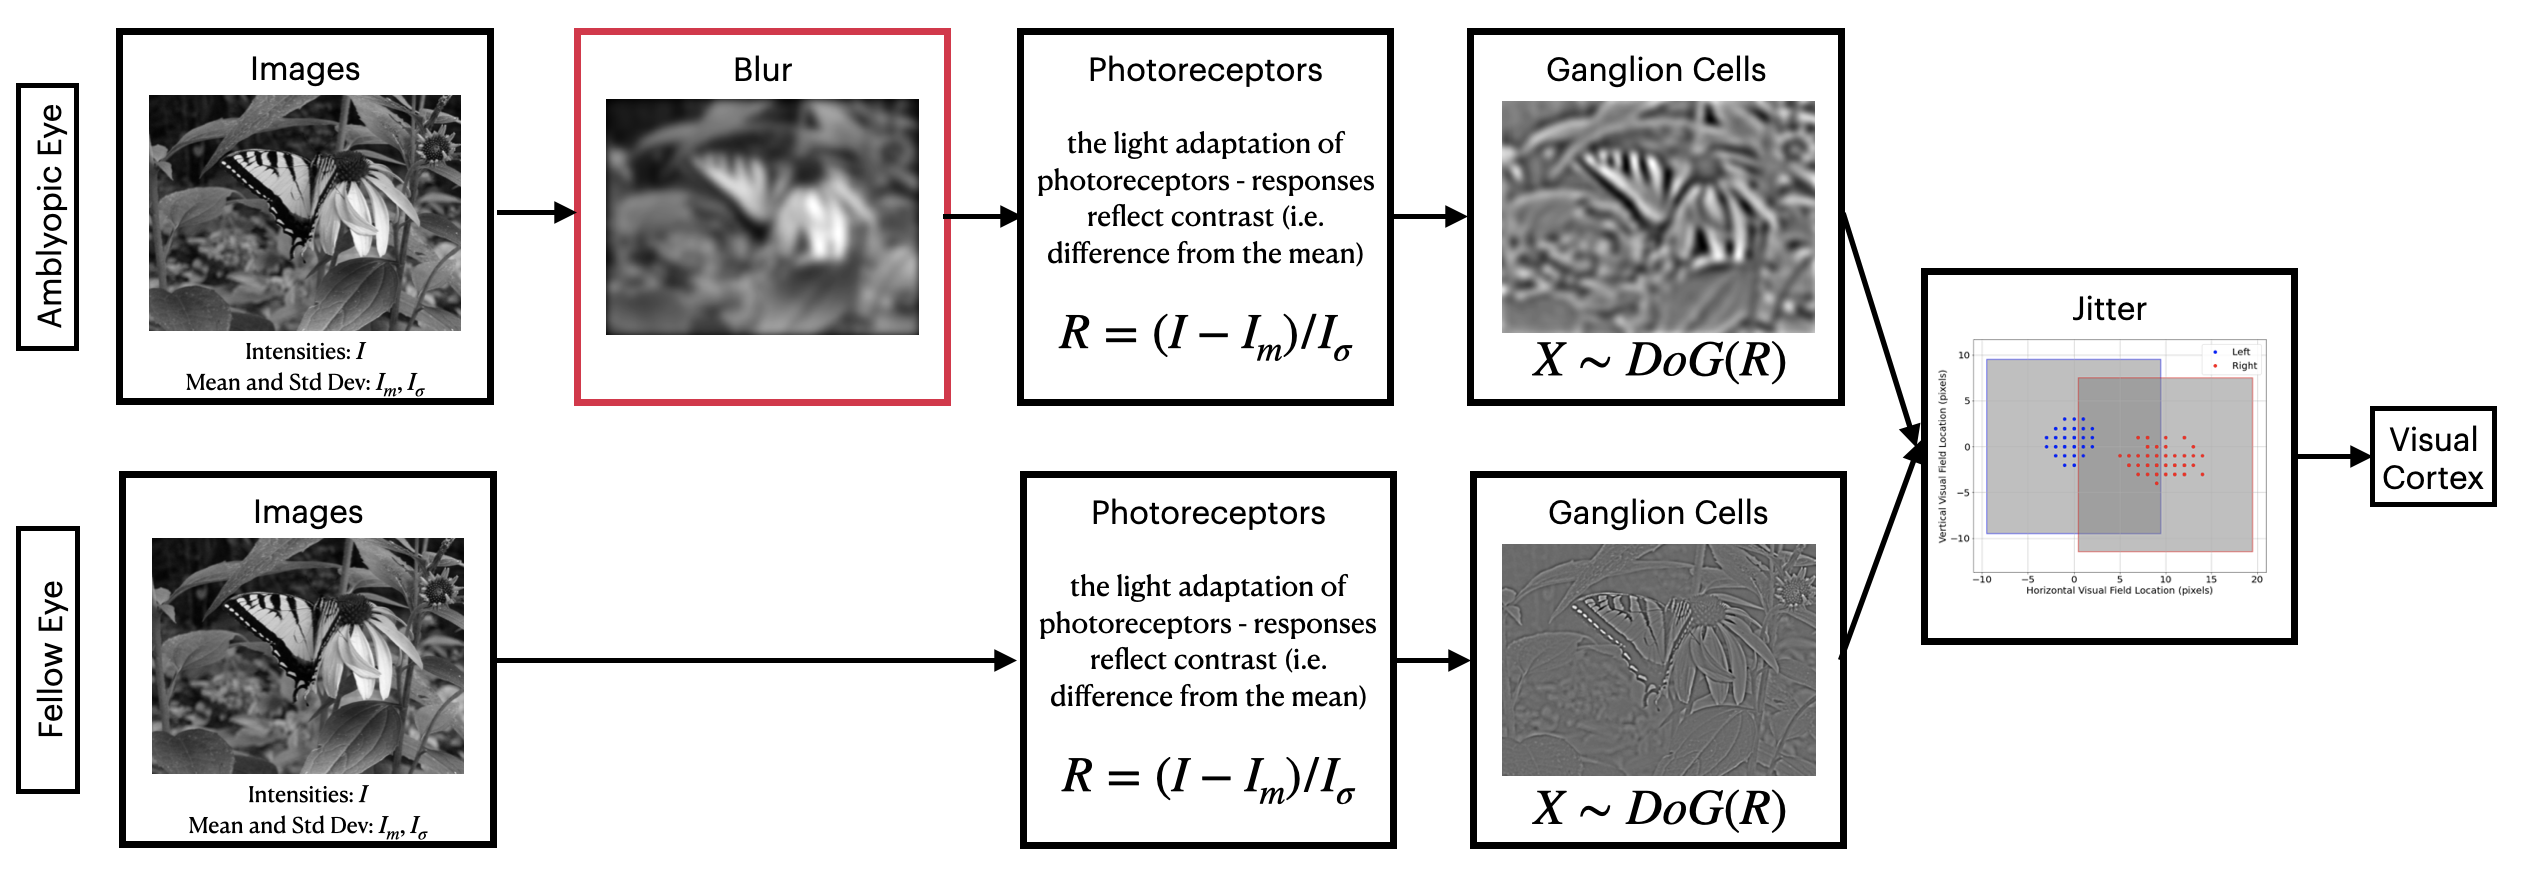
\includegraphics{/Users/bblais/Documents/Git/Amblyopia-Simulation/Manuscript/resources/Pasted image 20240301091305.png}
\caption{Vision Deficit Model.}\label{fig:vision_deficit_model}
\end{figure}

\begin{figure}
\centering
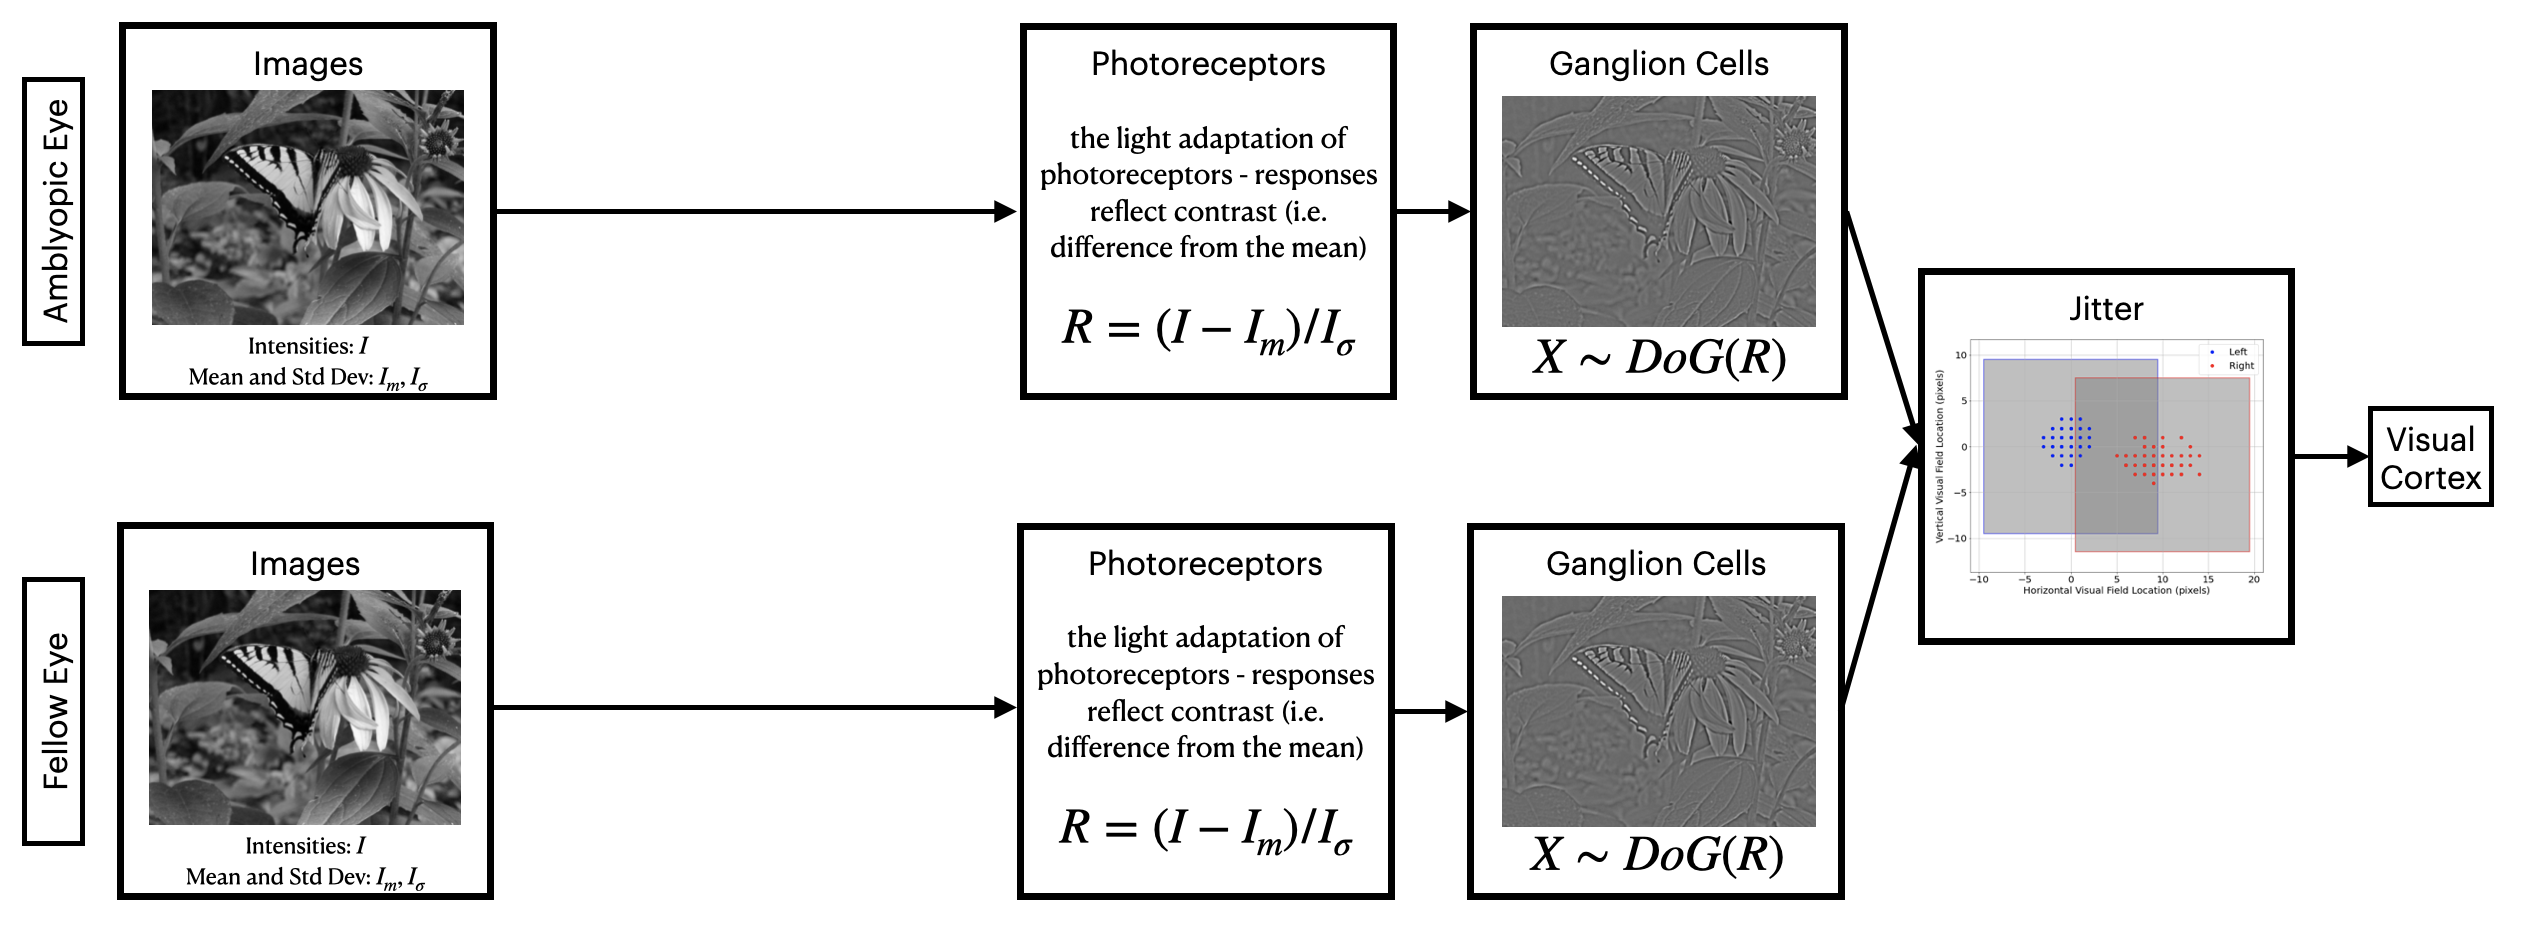
\includegraphics{/Users/bblais/Documents/Git/Amblyopia-Simulation/Manuscript/resources/Pasted image 20240301091503.png}
\caption{Optical Fix Model.}\label{fig:optical_fix_model}
\end{figure}

\begin{figure}
\centering
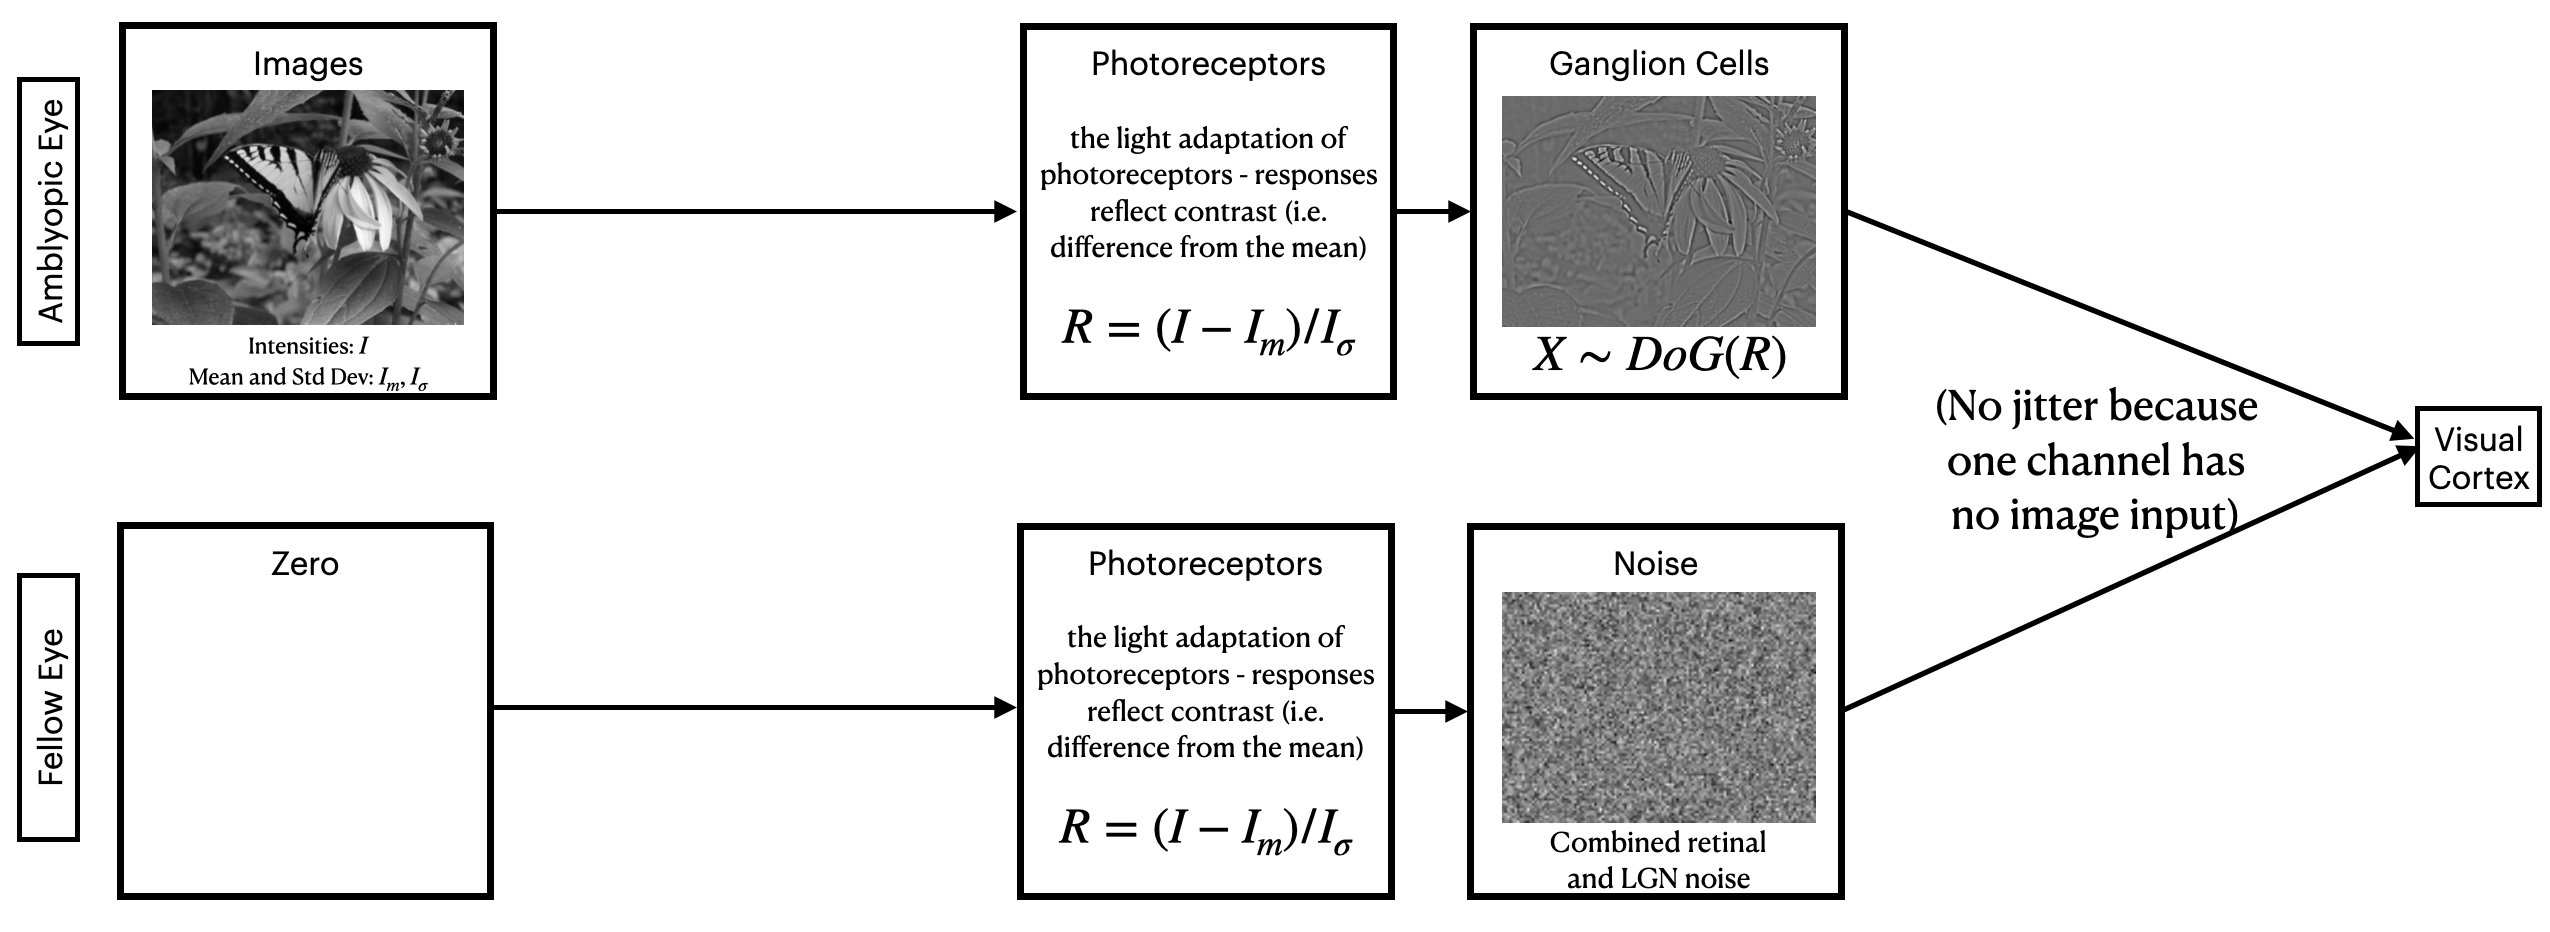
\includegraphics{/Users/bblais/Documents/Git/Amblyopia-Simulation/Manuscript/resources/Pasted image 20240301091523.png}
\caption{Patch Model.}\label{fig:patch_model}
\end{figure}

\begin{figure}
\centering
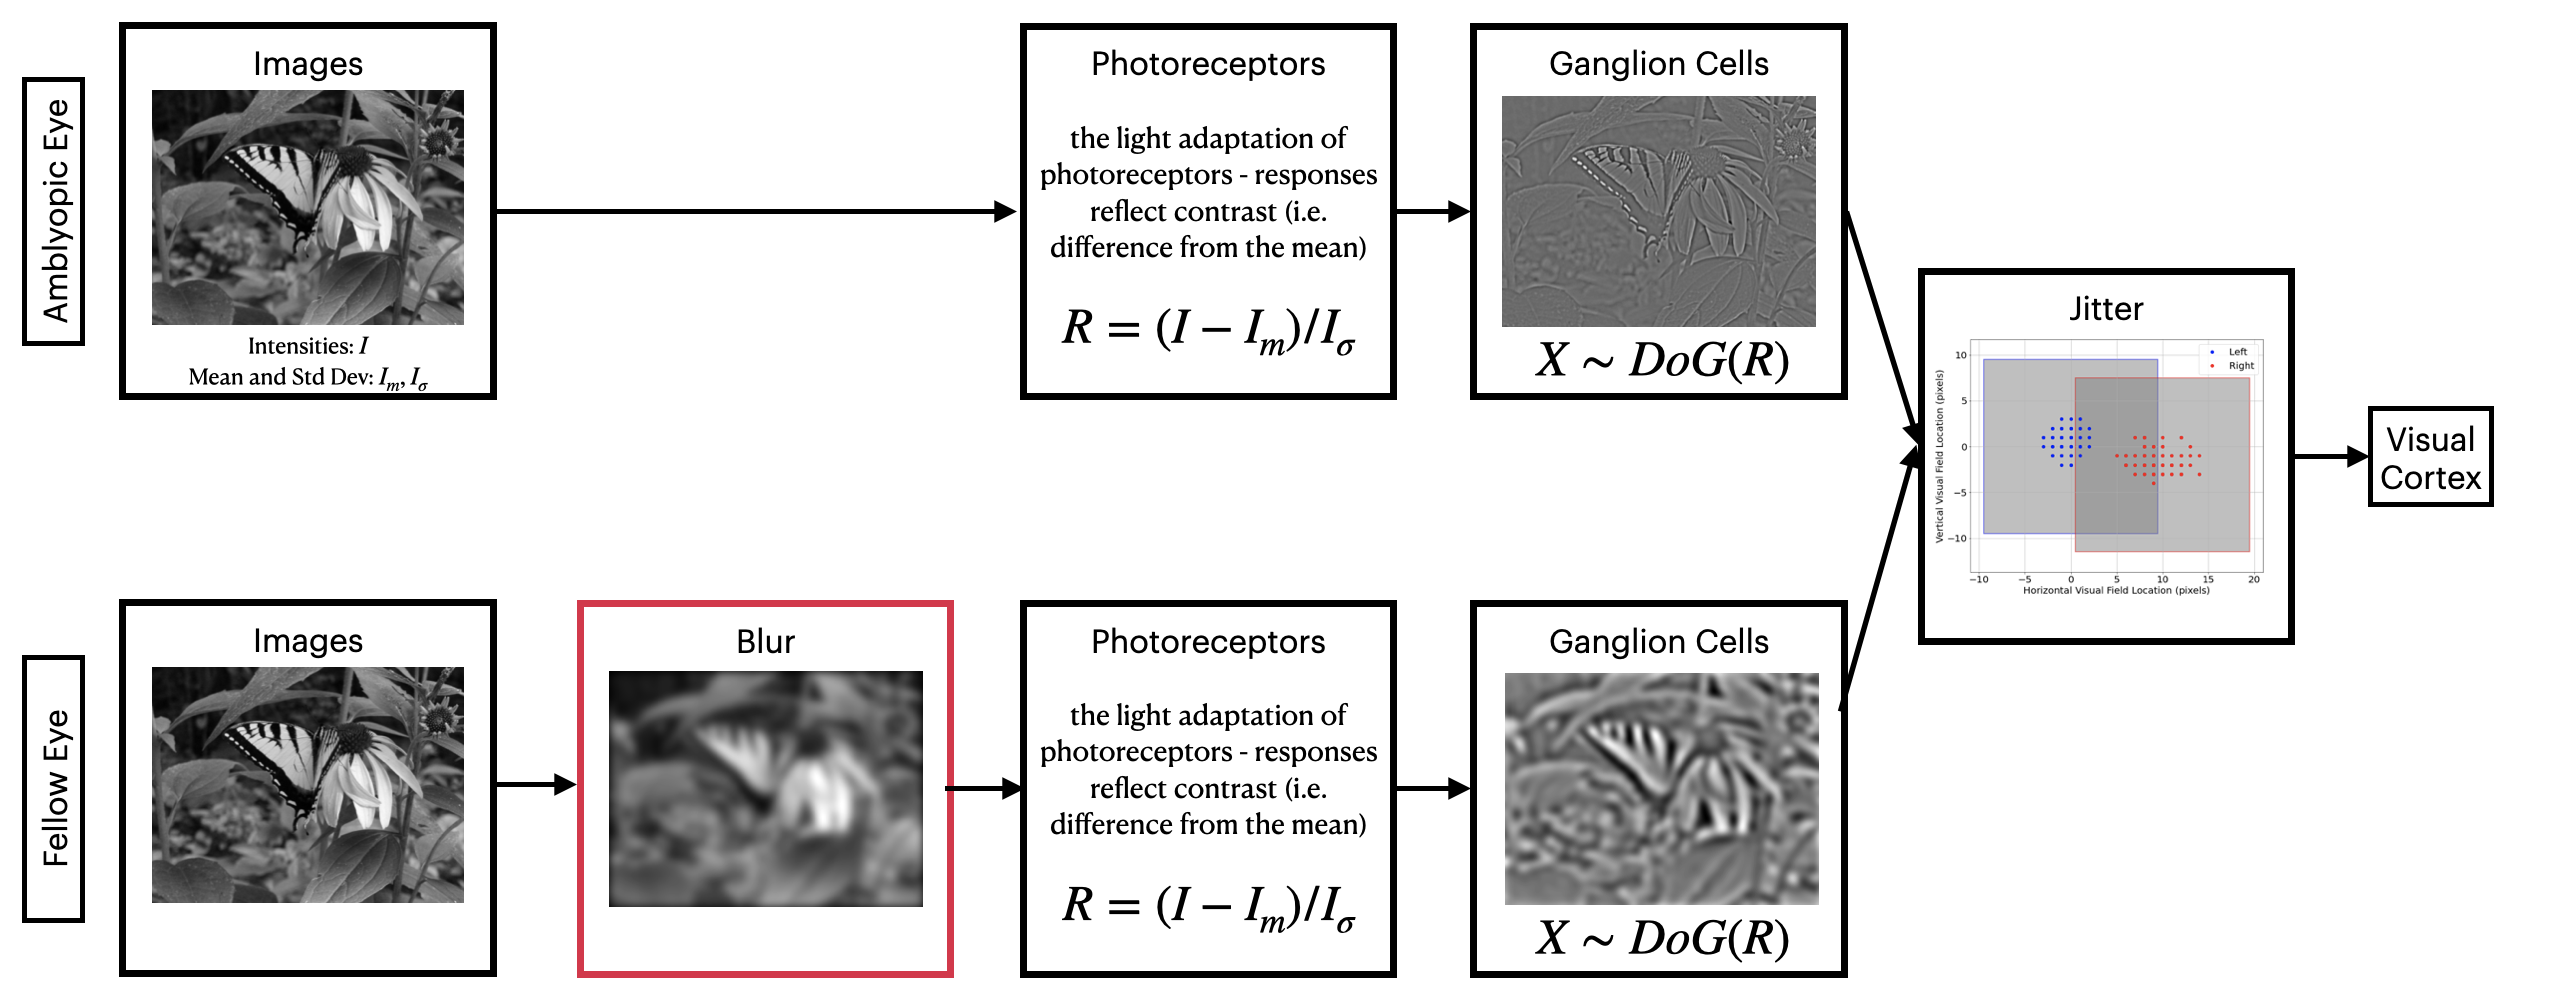
\includegraphics{/Users/bblais/Documents/Git/Amblyopia-Simulation/Manuscript/resources/Pasted image 20240301091538.png}
\caption{Atropine Model.}\label{fig:atropine_model}
\end{figure}

\begin{figure}
\centering
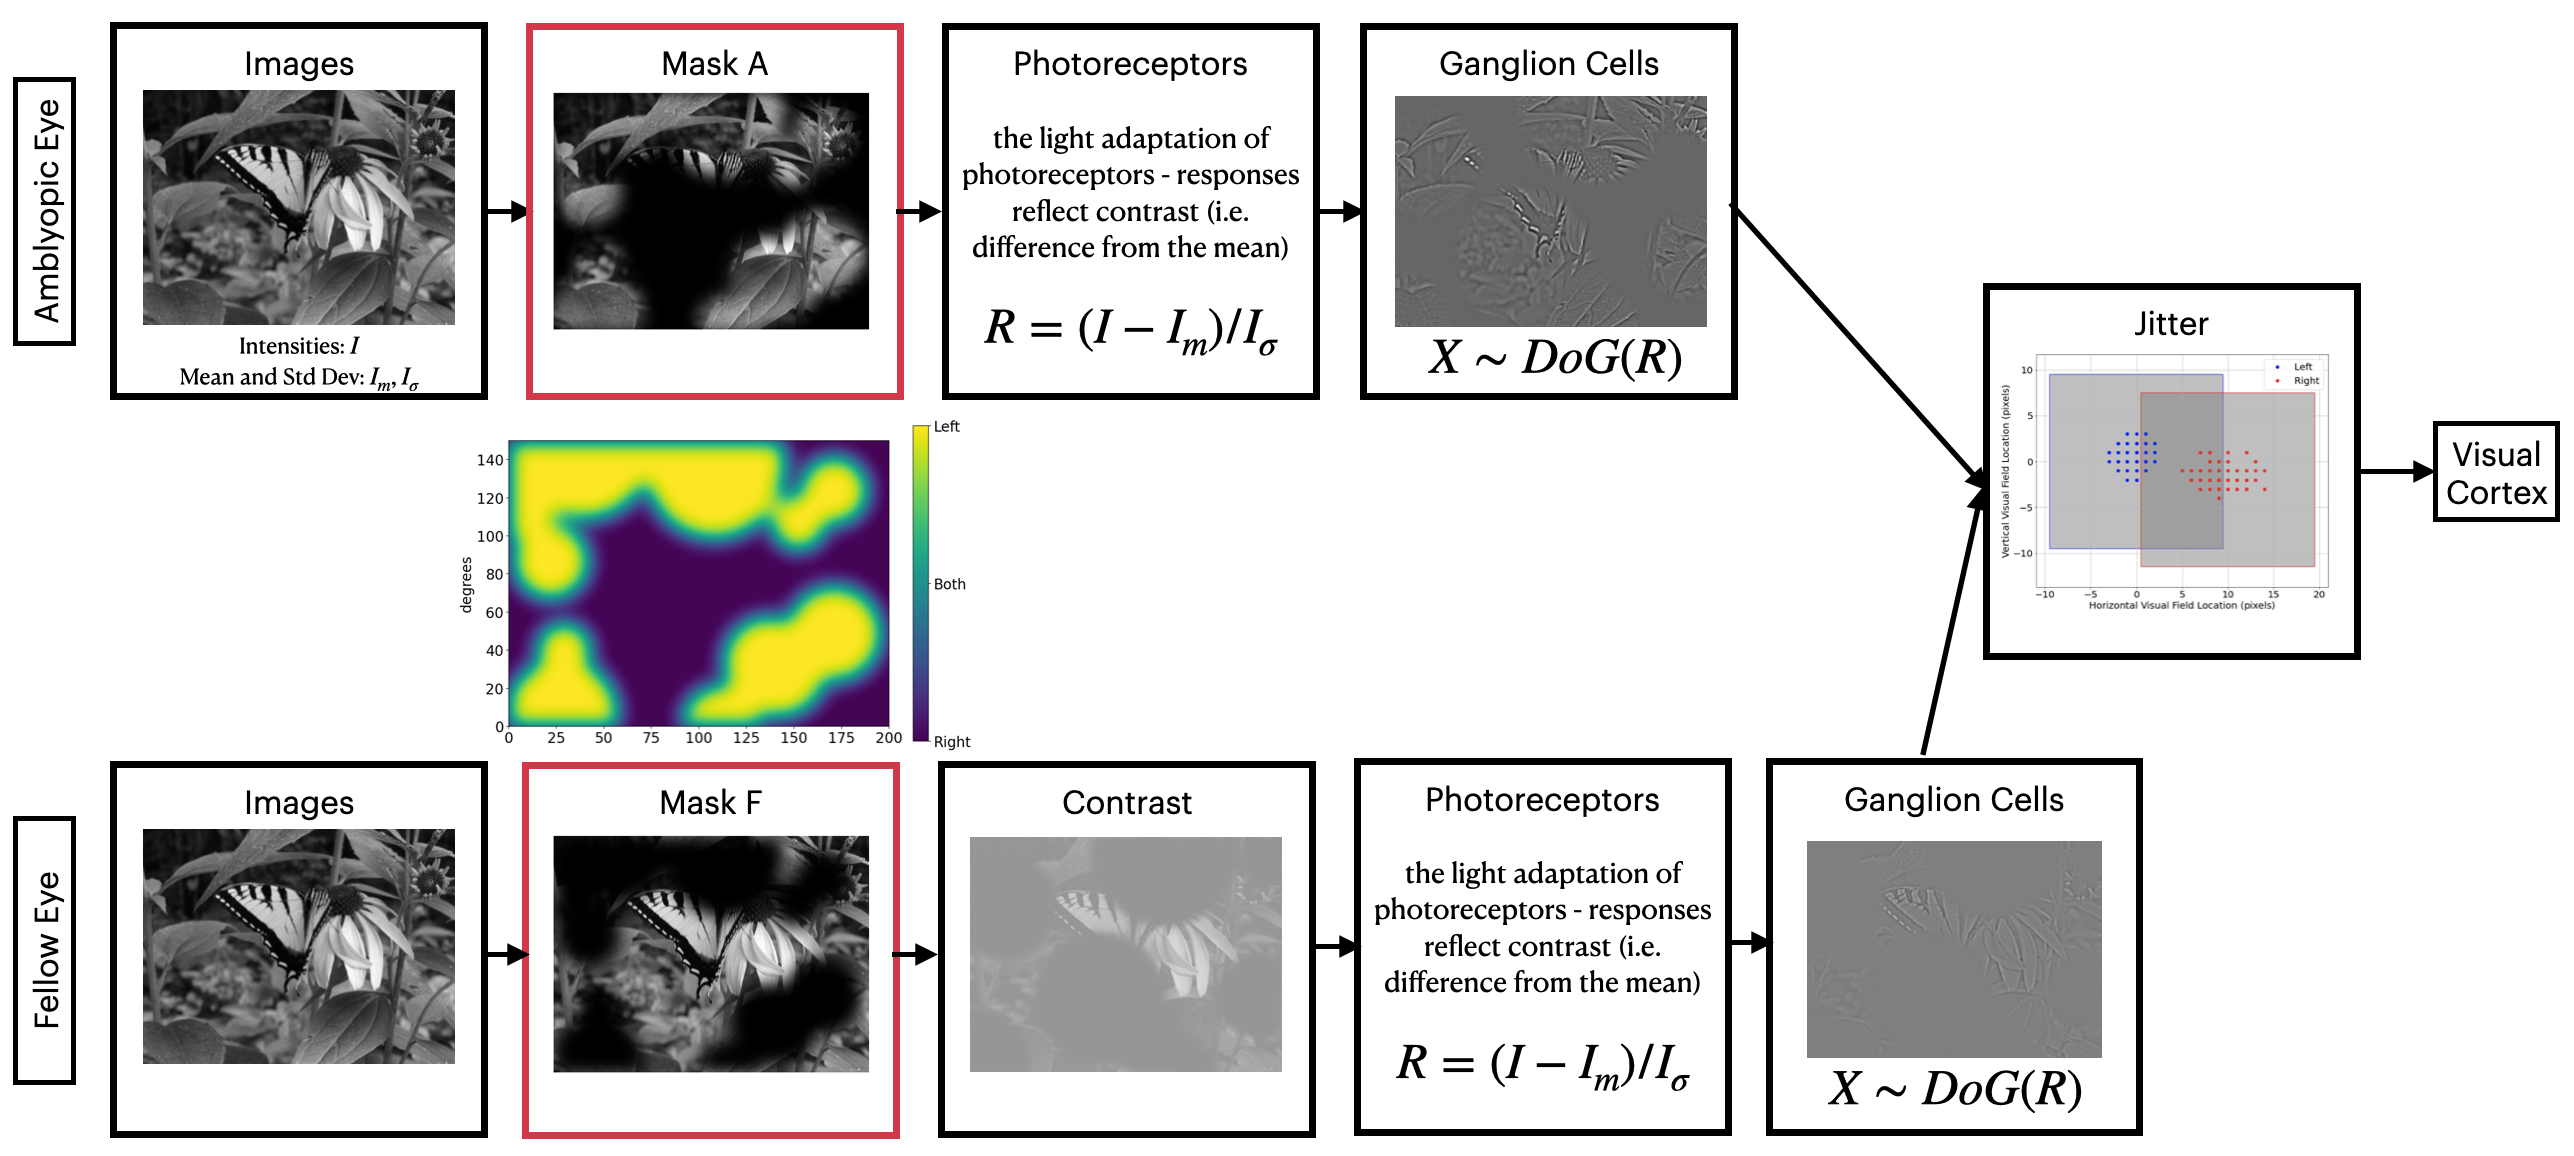
\includegraphics{/Users/bblais/Documents/Git/Amblyopia-Simulation/Manuscript/resources/Pasted image 20240301091600.png}
\caption{Contrast/Mask Model.}\label{fig:contrast_mask_model}
\end{figure}

\begin{figure}
\centering
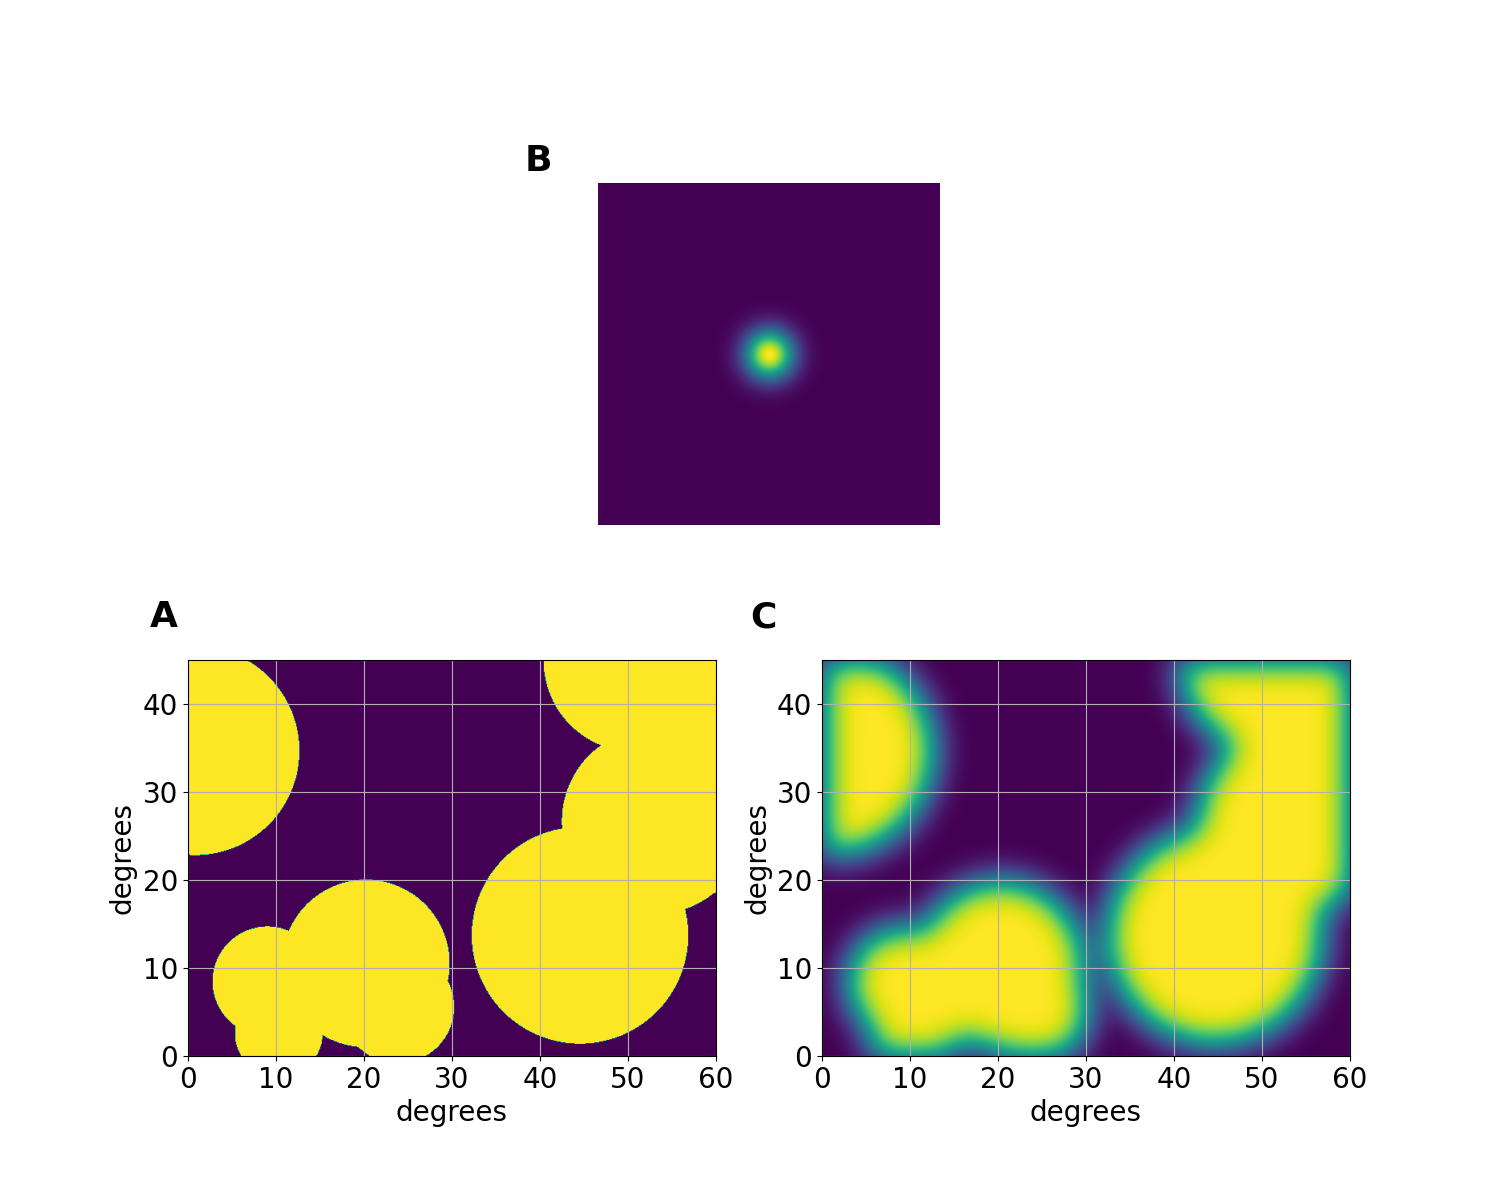
\includegraphics{/Users/bblais/Documents/Git/Amblyopia-Simulation/Manuscript/resources/blob_convolution_example_fsig_20.png}
\caption{Mask from blob.}\label{fig:dichopic_blob}
\end{figure}

\begin{figure}
\centering
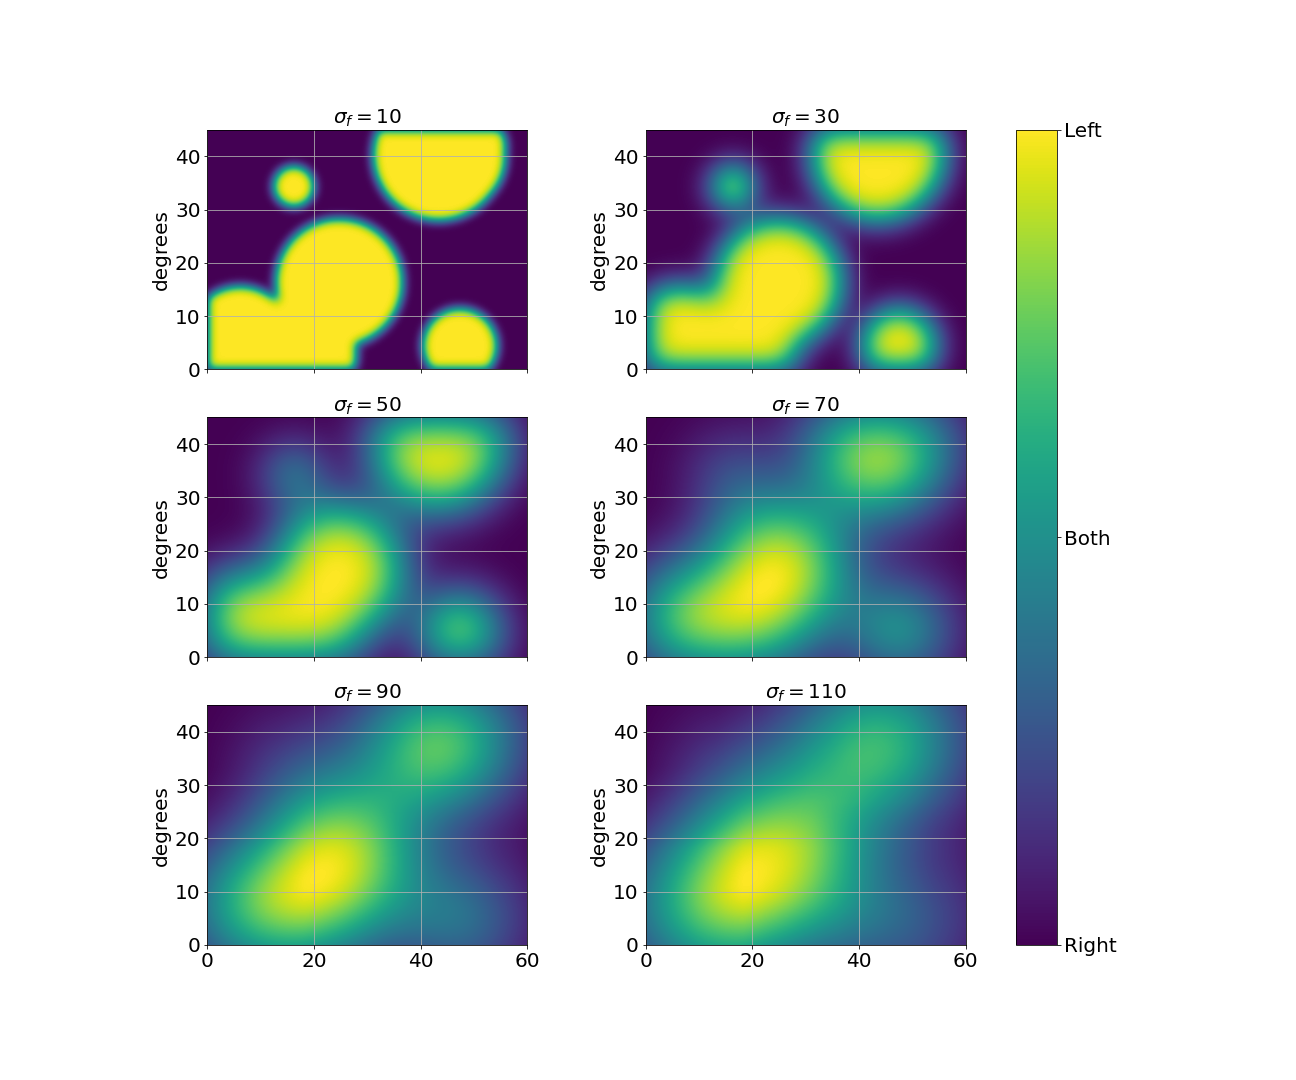
\includegraphics{/Users/bblais/Documents/Git/Amblyopia-Simulation/Manuscript/resources/mask_filter_examples_fsigs.png}
\caption{Mask filter size.}\label{fig:dichopic_filter_size}
\end{figure}

\begin{figure}
\centering
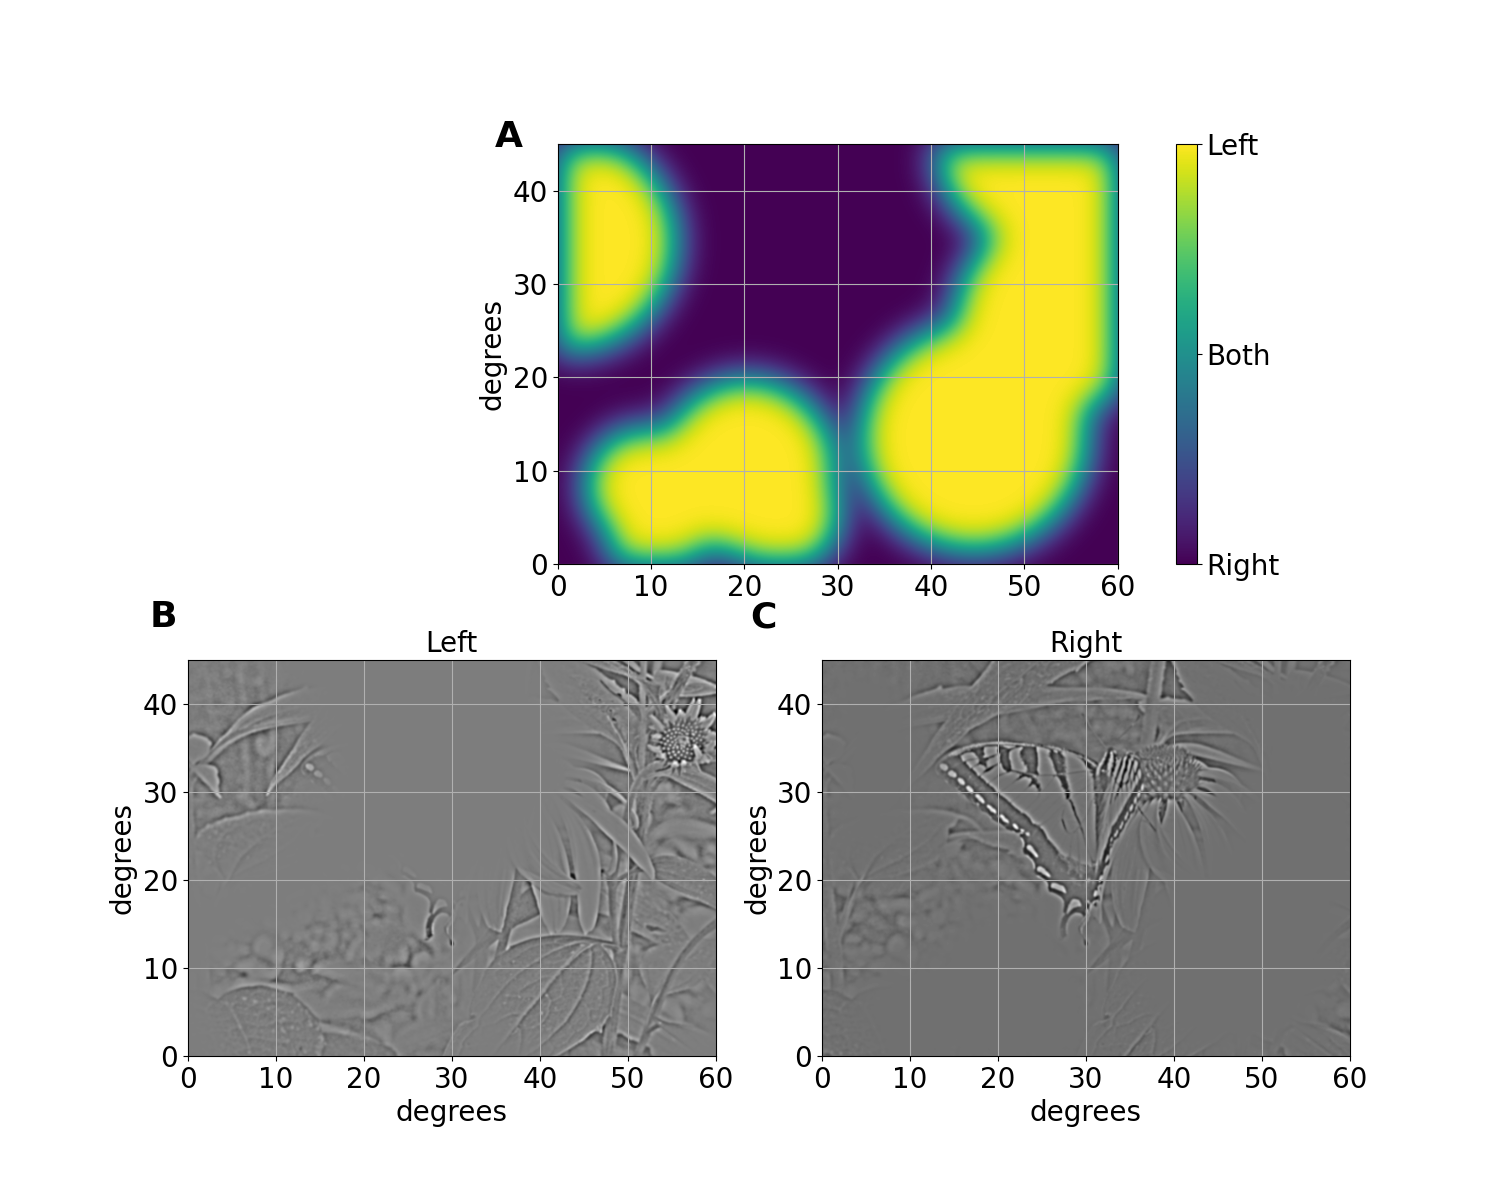
\includegraphics{/Users/bblais/Documents/Git/Amblyopia-Simulation/Manuscript/resources/mask_filter_example_fsig_20.png}
\caption{mask\_filter\_example\_fsig\_20.png}\label{figref:mask_filter_example_fsig_20.png}
\end{figure}

\section{Results on Modeling Visual
Deprivation}\label{sec:results-on-modeling-visual-deprivation}

\section{Results on Modeling Treatments for
Amblyopia}\label{sec:results-on-modeling-treatments-for-amblyopia}

As expected, the recovery from the deficit using the glasses treatment
depends on the open-eye noise, with greater recovery occurring for
larger noise level (Figure fig.~\ref{fig:glasses_treatment}). This is
due to the fact that larger presynaptic activity drives larger weight
changes, and the lack of structure in the noise drives the neuron to
find the structure in the now-identical eye inputs. The patch treatment
(Figure fig.~\ref{fig:patch_treatment}) has a larger effect on recovery,
again with larger noise resulting in faster recovery. The reason for the
enhanced recovery speed is that patch treatment sets up a direct
competition between the structure presented to the amblyopic eye and the
noise presented to the fellow eye.

Like patch, applying an atropine-like blur the fellow eye results in a
recovery (Figure fig.~\ref{fig:atropine_treatment}) that depends on the
noise level but also on the magnitude of the blur. For a sufficiently
larger blur, the patch and atropine treatments are roughly comparable.

\begin{figure}
\centering
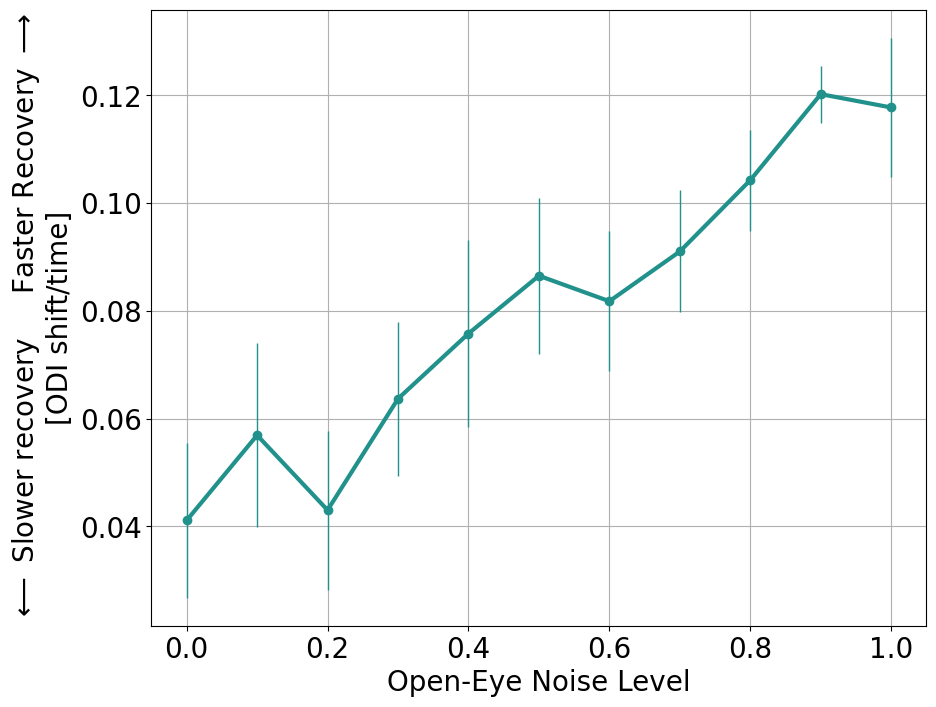
\includegraphics{/Users/bblais/Documents/Git/Amblyopia-Simulation/Manuscript/resources/Pasted image 20240529074233.png}
\caption{Glasses Treatment.}\label{fig:glasses_treatment}
\end{figure}

\begin{figure}
\centering
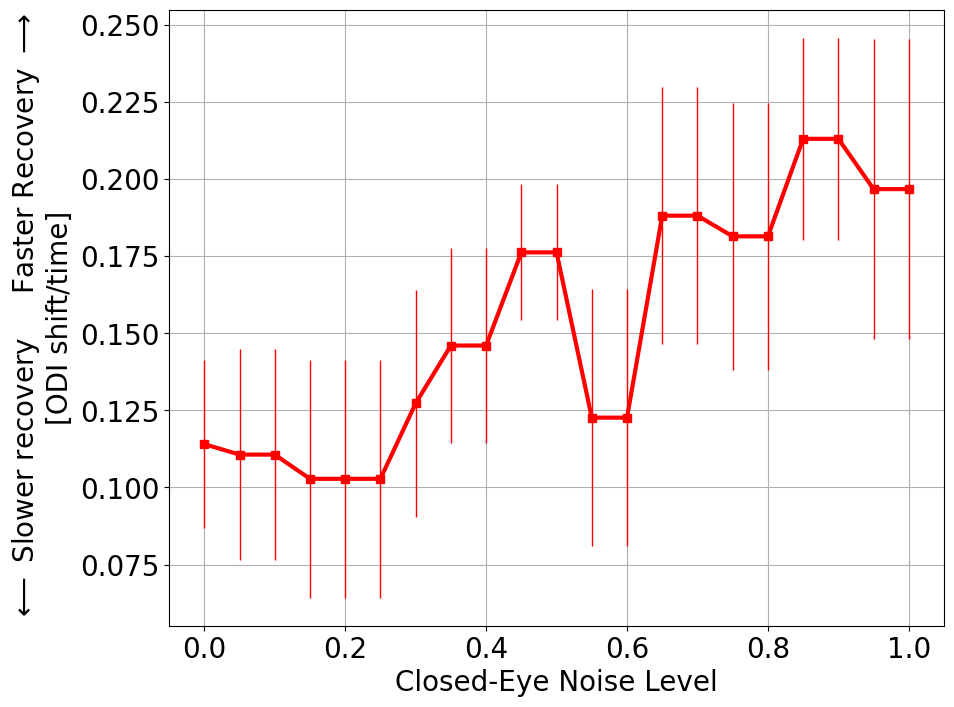
\includegraphics{/Users/bblais/Documents/Git/Amblyopia-Simulation/Manuscript/resources/Pasted image 20240529074250.png}
\caption{Patch Treatment.}\label{fig:patch_treatment}
\end{figure}

\begin{figure}
\centering
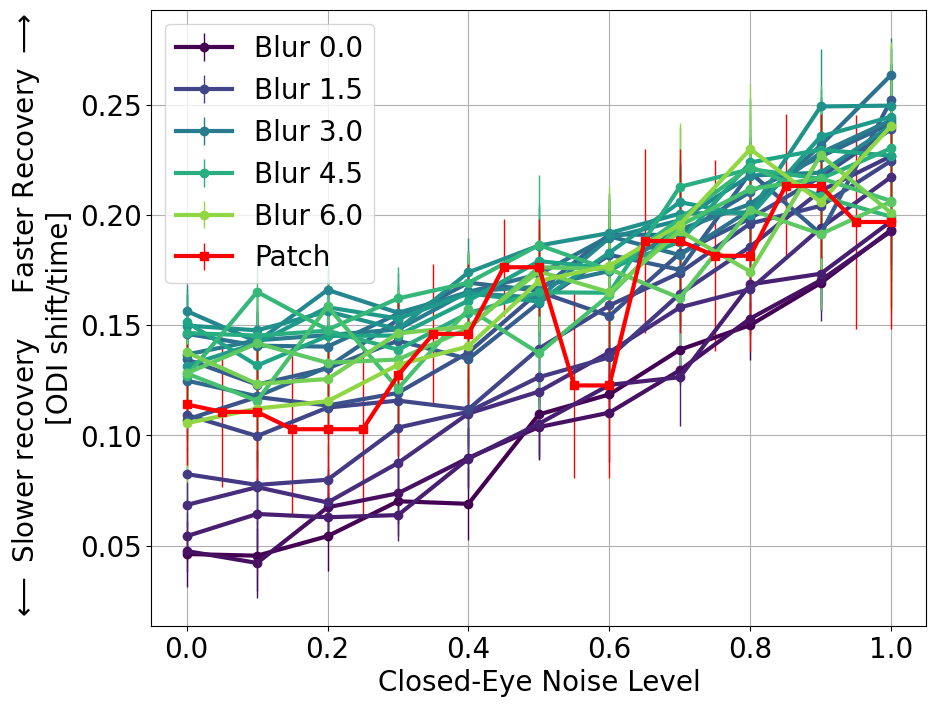
\includegraphics{/Users/bblais/Documents/Git/Amblyopia-Simulation/Manuscript/resources/Pasted image 20240529074320.png}
\caption{Patch Treatment.}\label{fig:atropine_treatment}
\end{figure}

Using a treatment constructed from a contrast reduction in the fellow
eye along with dichoptic masks can produce a recovery more pronounced
than any of the monocular treatments (Figure
fig.~\ref{fig:contrast_mask_treatment}). This recovery depends on the
level of contrast and the size of the mask, with smaller masks and a
contrast level around 0.3 being optimum. If the contrast difference is
not set low enough, the smaller mask enhances the competition between
the fellow eye and the amblyopic eye resulting in a \emph{worsening} of
the amblyopia. However contrast treatment alone doesn't provide an
optimal recovery -- the combination of both contrast reduction and the
dichoptic mask is needed. The result is surprisingly robust to eye
jitter (Figure fig.~\ref{fig:contrast_mask_treatment_mu9_sigma_9}) with
a mean jitter of half of the receptive field and a standard deviation of
the jitter equal to the mean giving the same effect, with only added
variation as the primary difference. There does seem to be in decrease
in range of contrasts which result in a worsening amblyopia, which may
be the result of the jitter giving a more variable deficit in the first
place and thus more options for recovery.

\begin{figure}
\centering
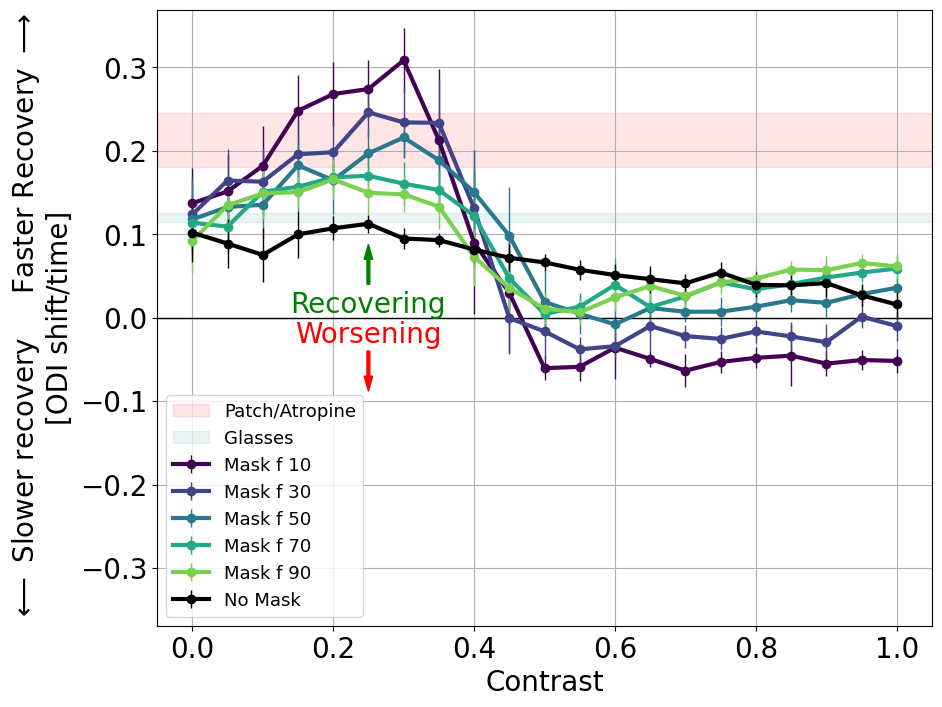
\includegraphics{/Users/bblais/Documents/Git/Amblyopia-Simulation/Manuscript/resources/Pasted image 20240529092844.png}
\caption{Contrast Treatment with Dichoptic
Mask}\label{fig:contrast_mask_treatment}
\end{figure}

\begin{figure}
\centering
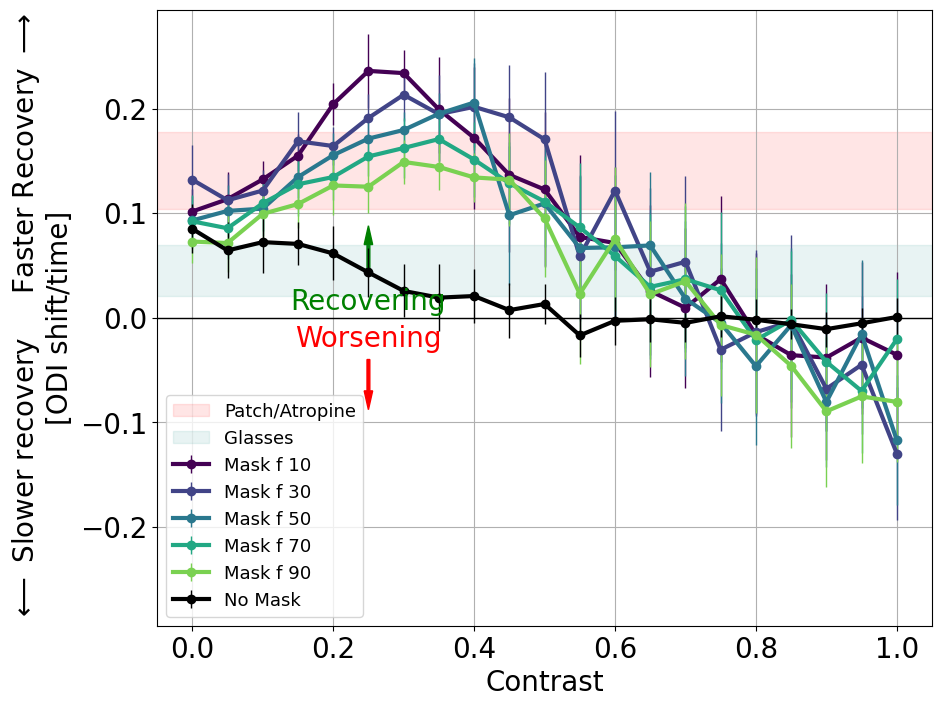
\includegraphics{/Users/bblais/Documents/Git/Amblyopia-Simulation/Manuscript/resources/Pasted image 20240529094751.png}
\caption{Contrast Treatment with Dichoptic Mask with jitter \(\mu_c=9\),
\(\sigma_c=9\).}\label{fig:contrast_mask_treatment_mu9_sigma_9}
\end{figure}

\#todo - {[} {]} do the same sims with the min activity at 0.5

\section*{References}\label{sec:references}
\addcontentsline{toc}{section}{References}

\phantomsection\label{refs}
\begin{CSLReferences}{0}{1}
\bibitem[\citeproctext]{ref-BCM82}
\CSLLeftMargin{1. }%
\CSLRightInline{Bienenstock, E.L., Cooper, L.N., and Munro, P.W. (1982).
Theory for the development of neuron selectivity: Orientation
specificity and binocular interaction in visual cortex. Journal of
Neuroscience \emph{2}, 32--48.}

\bibitem[\citeproctext]{ref-phd:Blais98}
\CSLLeftMargin{2. }%
\CSLRightInline{Blais, B.S. (1998). The role of the environment in
synaptic plasticity:\\
towards an understanding of learning and memory.}

\bibitem[\citeproctext]{ref-IntratorCooper92}
\CSLLeftMargin{3. }%
\CSLRightInline{Intrator, N., and Cooper, L.N. (1992).
\href{ftp://cns.brown.edu/nin/papers/cooper.ps.Z}{Objective function
formulation of the {BCM} theory of visual cortical plasticity:
Statistical connections, stability conditions}. Neural Networks
\emph{5}, 3--17.}

\bibitem[\citeproctext]{ref-LawCooper94}
\CSLLeftMargin{4. }%
\CSLRightInline{Law, C., and Cooper, L. (1994). Formation of receptive
fields according to the {BCM} theory in realistic visual environments.
Proceedings National Academy of Sciences \emph{91}, 7797--7801.}

\bibitem[\citeproctext]{ref-brito2024learning}
\CSLLeftMargin{5. }%
\CSLRightInline{Brito, C.S.N. de, and Gerstner, W. (2024). Learning what
matters: Synaptic plasticity with invariance to second-order input
correlations. PLOS Computational Biology \emph{20}, e1011844.}

\bibitem[\citeproctext]{ref-BlaisEtAl99}
\CSLLeftMargin{6. }%
\CSLRightInline{Blais, B., Shouval, H., and Cooper, L.N. (1999). The
role of presynaptic activity in monocular deprivation: Comparison of
homosynaptic and heterosynaptic mechanisms. Proc. Natl. Acad. Sci.
\emph{96}, 1083--1087.}

\bibitem[\citeproctext]{ref-JeonEtAl1998}
\CSLLeftMargin{7. }%
\CSLRightInline{Jeon, C.J., Strettoi, E., and Masland, R.H. (1998). {The
major cell populations of the mouse retina}. J Neurosci \emph{18},
8936--8946.}

\bibitem[\citeproctext]{ref-SterlingEtAl1988}
\CSLLeftMargin{8. }%
\CSLRightInline{Sterling, P., Freed, M.A., and Smith, R.G. (1988).
{Architecture of rod and cone circuits to the on-beta ganglion cell}. J
Neurosci \emph{8}, 623--642.}

\bibitem[\citeproctext]{ref-hubel1995eye}
\CSLLeftMargin{9. }%
\CSLRightInline{Hubel, D.H. (1995). Eye, brain, and vision. (Scientific
American Library/Scientific American Books).}

\bibitem[\citeproctext]{ref-bonin2005suppressive}
\CSLLeftMargin{10. }%
\CSLRightInline{Bonin, V., Mante, V., and Carandini, M. (2005). The
suppressive field of neurons in lateral geniculate nucleus. Journal of
Neuroscience \emph{25}, 10844--10856.}

\bibitem[\citeproctext]{ref-carandini2012normalization}
\CSLLeftMargin{11. }%
\CSLRightInline{Carandini, M., and Heeger, D.J. (2012). Normalization as
a canonical neural computation. Nature Reviews Neuroscience \emph{13},
51--62.}

\bibitem[\citeproctext]{ref-glaser2002randomized}
\CSLLeftMargin{12. }%
\CSLRightInline{Glaser, S.R., Matazinski, A.M., Sclar, D.M., Sala, N.A.,
Vroman, C.M., Tanner, C.E., Stager, D.R., Berry, P.M., Felius, J.,
Wilkerson, J.A., et al. (2002). A randomized trial of atropine vs
patching for treatment of moderate amblyopia in children. Archives of
ophthalmology \emph{120}, 268--278.}

\bibitem[\citeproctext]{ref-xiao2020improved}
\CSLLeftMargin{13. }%
\CSLRightInline{Xiao, S., Gaier, E.D., Mazow, M.L., Stout, A.U.,
Travers, D.A., Angjeli, E., Wu, H.C., Binenbaum, G., and Hunter, D.G.
(2020). Improved adherence and treatment outcomes with an engaging,
personalized digital therapeutic in amblyopia. Scientific Reports
\emph{10}, 1--8.}

\bibitem[\citeproctext]{ref-Li:2015aa}
\CSLLeftMargin{14. }%
\CSLRightInline{Li, S.L., Reynaud, A., Hess, R.F., Wang, Y.-Z., Jost,
R.M., Morale, S.E., De La Cruz, A., Dao, L., Stager, D., Jr, and Birch,
E.E. (2015). Dichoptic movie viewing treats childhood amblyopia. J AAPOS
\emph{19}, 401--405.
\url{https://doi.org/10.1016/j.jaapos.2015.08.003}.}

\bibitem[\citeproctext]{ref-xiao2022randomized}
\CSLLeftMargin{15. }%
\CSLRightInline{Xiao, S., Angjeli, E., Wu, H.C., Gaier, E.D., Gomez, S.,
Travers, D.A., Binenbaum, G., Langer, R., Hunter, D.G., Repka, M.X., et
al. (2022). Randomized controlled trial of a dichoptic digital
therapeutic for amblyopia. Ophthalmology \emph{129}, 77--85.}

\end{CSLReferences}

\end{document}
